% =============================================================================
% HoloQPI manuscript, version 4.2 (corrected crop origin and in-line pairing)
%
% Compile with BibTeX:
%     pdflatex main.tex && bibtex main && pdflatex main.tex && pdflatex main.tex
%
% Every number comes from the corrected result files under runs/ and logs/ via
% results_for_manuscript/ (built by analysis/v42/compile_results.py). Tables 3-7
% and 10-11 were brought in line with it by analysis/v42/update_tables.py; the
% registration values of Sec. 4.1 come from the diagnostics archive
% (diagnostics/registration_summary.json, hologram_registration.csv), which is not
% part of the repository. Table 1 is the dataset composition. The numbers in the
% tables and in the text are checked by analysis/v42/check_numbers.py
% (output: analysis/v42/check_numbers.csv).
% =============================================================================
\documentclass[11pt]{article}

\usepackage[a4paper,margin=1in]{geometry}
\usepackage{mathptmx}
\usepackage{amsmath}
\usepackage{amssymb}
\usepackage{graphicx}
\usepackage{enumitem}
\usepackage{booktabs}
\usepackage{array}
\usepackage{tabularx}
\usepackage{multirow}
\usepackage[font=small,labelfont=bf,width=\textwidth,skip=4pt]{caption}
\usepackage{subcaption}
\usepackage{xcolor}
\usepackage[hidelinks]{hyperref}
\usepackage{url}
\usepackage{cite}
\usepackage{microtype}
\usepackage{flafter}
\usepackage[section]{placeins}
\usepackage{setspace}
\setstretch{1.12}

\renewcommand{\topfraction}{0.85}
\renewcommand{\bottomfraction}{0.6}
\renewcommand{\textfraction}{0.12}
\renewcommand{\floatpagefraction}{0.75}
\setcounter{topnumber}{2}
\setcounter{bottomnumber}{2}
\setcounter{totalnumber}{4}
\setlength{\textfloatsep}{14pt plus 2pt minus 4pt}
\setlength{\floatsep}{12pt plus 2pt minus 2pt}

% Table style: every table spans \textwidth, uses \footnotesize, and keeps
% notes to symbol definitions.
\newcommand{\tabnote}[1]{\par\vspace{2pt}{\raggedright\footnotesize #1\par}}
\setlength{\tabcolsep}{4pt}

\graphicspath{{manuscript_images/}{figures/}}

\usepackage{titlesec}
\titleformat{\section}{\normalfont\large\bfseries}{\thesection}{0.6em}{}
\titleformat{\subsection}{\normalfont\normalsize\bfseries}{\thesubsection}{0.6em}{}
\titleformat{\subsubsection}{\normalfont\normalsize\itshape}{\thesubsubsection}{0.6em}{}
\titlespacing*{\section}{0pt}{1.4ex plus 0.6ex minus 0.3ex}{0.8ex}
\titlespacing*{\subsection}{0pt}{1.1ex plus 0.5ex minus 0.3ex}{0.5ex}
\titlespacing*{\subsubsection}{0pt}{0.9ex plus 0.4ex minus 0.2ex}{0.4ex}

\newcommand{\Lphase}{\mathcal{L}_\mathrm{phase}}
\newcommand{\Lseg}{\mathcal{L}_\mathrm{seg}}
\newcommand{\Lippc}{\mathcal{L}_\mathrm{IPP}^\mathrm{cell}}
\newcommand{\Lippi}{\mathcal{L}_\mathrm{IPP}^\mathrm{img}}
\newcommand{\Larea}{\mathcal{L}_\mathrm{area}}
\newcommand{\Lbga}{\mathcal{L}_\mathrm{BGA}}
\newcommand{\Lfwd}{\mathcal{L}_\mathrm{fwd}}
\newcommand{\Lamp}{\mathcal{L}_\mathrm{amp}}

\title{\bfseries Joint Phase Reconstruction and Cell Segmentation from Raw
Holograms for Per-Cell Dry-Mass Measurement}

\author{Usama Ikram\quad Inkyu Moon\\[2pt]
\normalsize Department of Robotics and Mechatronics Engineering,\\
\normalsize Daegu Gyeongbuk Institute of Science and Technology (DGIST),
Daegu, Republic of Korea}

\date{}

% =============================================================================
\begin{document}
\maketitle

\begin{abstract}
\noindent
Per-cell dry mass in quantitative phase imaging is the phase integrated over a
segmented cell, so its accuracy depends on the reconstructed phase and on the
cell boundary together. We trained a network of 9.6\,M parameters, a
MobileNetV2 encoder with two U-Net-style decoders, that maps a raw digital
hologram to a quantitative phase map and a cell segmentation, and we scored
every prediction through a fixed per-cell measurement chain as well as with
phase and segmentation metrics. Segmentation labels were derived from the
reference phase. On the off-axis test set (113 fields, 3186 reference cells,
three training seeds), the dry-mass mean absolute percentage error (MAPE) over
matched cells was $0.1742$, against $0.2203$ for the tested classical
reconstruction pipeline, at similar Dice ($0.8337$ and $0.8253$) and
projected-area MAPE ($0.1568$ and $0.1578$). On the same test set, detection
recall was $0.593$ overall, $0.912$ for interior reference cells and $0.212$ for
cells within 3\,px of the field boundary, and for matched cells the error lay
in the predicted phase level rather than in the predicted cell domain. On the
107 test fields whose in-line Gabor hologram is correctly paired with the
reference (3055 reference cells), a single in-line training run reached a phase
Pearson $r$ of $0.8667$ and a dry-mass MAPE of $0.2129$; the tested classical
in-line reconstruction did not recover the specimen phase ($r=-0.2075$). On the
off-axis test set, both measurement-aware integrated-phase terms increased the
matched-cell dry-mass MAPE ($+0.0141$ per cell and $+0.0145$ per image, both
resolved under a between-seed criterion), and their effect on the field-total
error was not resolved. The forward-model consistency term did not resolve the
phase scale under the implemented operator and did not constrain the off-axis
propagation distance, whereas the in-line residual had its minimum at the
recording distance. Displacing every reference boundary outward by one pixel,
with no trained model involved, changed dry mass by $4.8\%$ while Dice stayed at
$0.974$.
\end{abstract}

\vspace{0.6em}

% =============================================================================
\section{Introduction}
\label{sec:intro}

Quantitative phase imaging measures the optical path length that a specimen
adds to the illumination. For a cell this path length is proportional to the
dry mass of its non-aqueous content~\cite{barer1952,zangle2014,lee2013qpi}, so
a per-cell measurement in digital holographic microscopy (DHM) comes out of a
chain of steps: the hologram is reconstructed into a phase map, each cell is
delineated, and the phase is integrated inside each boundary. Dry mass is the
product of a phase level and an integration domain. A phase map that is biased
inside cells gives a biased mass through a correct boundary, and a correct phase
map gives a biased mass through a boundary placed a pixel or two off. The scale
of the second effect can be measured without any trained model: on the test
fields used here, moving every reference boundary outward by one pixel changes
dry mass by $4.8\%$ while Dice stays at $0.974$ (Sec.~\ref{sec:res-boundary}).
Image-level statistics can also cancel the errors that a per-cell measurement
is sensitive to: if one cell in a field is over-estimated by 20\% and another is
under-estimated by 20\%, the field total is unbiased. Whether a reconstruction
or a segmentation is adequate for quantitative work therefore has to be judged
on the measurement itself.

The classical reconstruction chain has several stages, each with its own
parameters, typically sideband filtering, phase unwrapping, aberration
compensation and refocusing~\cite{zhao2023vynet,wen2025rbf,bai2026macrophage}.
A recent review of learned methods in DHM organises the field along the same
stages, with networks used for phase reconstruction and, separately, for
analysis of the reconstructed phase~\cite{moon2026aidhm}. Networks that take
the recorded hologram as input can replace the reconstruction with a single
forward pass~\cite{di2021phasenet,jaferzadeh2022holophasenet,zhao2023vynet,delikoyun2025rthad},
or skip it for a downstream task such as detection, counting or
classification~\cite{trujillo2019automatic,wen2026direct,delikoyun2025rthad}.
Among the learned reconstruction studies we reviewed, the output is mostly
scored against the classical phase with image criteria: SSIM, the fraction of
pixels within a phase tolerance, or mean absolute
error~\cite{di2021phasenet,zhao2023vynet,delikoyun2025rthad}. Two of them also
compared cell measurements obtained from network and reference images, as
distributions over the test cells~\cite{jaferzadeh2022holophasenet,park2026ai}.
A roadmap on holographic QPI called for metrology studies of network-formed
phase images before such images are accepted for quantitative
imaging~\cite{balasubramani2021roadmap}.

In most of the studies we examined, cells are segmented for per-cell
measurement on phase that was reconstructed beforehand, either with classical
rules~\cite{shen2022laf,bai2026macrophage,kyeremah2025malaria} or with trained
networks~\cite{li2025dlcspf,park2025holofluonet}. Analysis directly on the
hologram has also been reported. A convolutional network detected and counted
red blood cells in raw off-axis holograms~\cite{trujillo2019automatic}, a U-Net
segmented cells on raw off-axis holograms with Dice and IoU of about
0.5~\cite{wen2026direct}, and a network trained on simulated in-line holograms
of microplankton predicts segmentation and dry-mass maps from the raw
hologram~\cite{bachimanchi2022microplankton}. Two systems cover more of the
chain. In one, a single-shot Gabor hologram is mapped to quantitative phase and
virtual fluorescence, per-cell measurements are extracted both with
segmentation of the phase image and with membrane-fluorescence segmentation
applied to the phase; measurements from generated and ground-truth images are
compared as distributions, and the generated measurements are used for
cell-type and drug-response classification~\cite{park2026ai}.
In the other, an imaging flow cytometer chains a learned off-axis
reconstruction with a cell detector and an aggregate
analysis~\cite{delikoyun2025rthad}.

The components of a raw-hologram-to-measurement pipeline, and several partial
combinations of them, therefore exist in prior work. In the studies reviewed
here, we did not find paired per-cell measurement errors reported together with
detection coverage. Nor did we identify a study that tests whether an explicit
measurement term or a forward-model consistency term, added to a supervised
objective, reduces the paired per-cell measurement error on experimental
holographic data.

This study examines one network that takes a raw hologram and jointly predicts
quantitative phase, a cell segmentation and, optionally, the transmitted
amplitude. A fixed measurement chain computes per-cell quantities from these
outputs, and no classical reconstruction enters the inference path. We keep
three levels of evaluation separate: the network outputs (phase and amplitude
error, segmentation overlap), cell detection and geometry (recall, precision,
projected area, circularity), and the quantitative measurements (integrated
phase and dry mass). The reference segmentation is derived from the reference
phase by a fixed thresholding rule, so segmentation, detection and matched-cell
results are relative to phase-derived labels.

\noindent The main contributions of this work are:
\begin{enumerate}[leftmargin=*, itemsep=2pt, topsep=3pt]
\item An evaluation of a joint raw-hologram-to-phase-and-mask network, built
from a MobileNetV2 encoder~\cite{sandler2018mobilenetv2} and U-Net-style
decoders~\cite{ronneberger2015unet}, by the paired per-cell error of matched
cells, reported with detection recall, a coverage-adjusted error and field
totals, and split into a domain factor and a phase factor
(Secs.~\ref{sec:eval} and~\ref{sec:res-measure}).
\item A comparison with one specified classical reconstruction pipeline through
the same measurement chain, off-axis on 113 test fields and for both geometries
on the 107 fields whose in-line hologram is correctly paired
(Sec.~\ref{sec:res-recon}).
\item Tests of measurement-aware integrated-phase objectives with three training
seeds per configuration, and of a forward-model consistency term, including its
sensitivity to the phase scale and to the propagation distance in both
geometries (Secs.~\ref{sec:res-mawo} and~\ref{sec:res-fwd}).
\item A model-free analysis of how boundary displacement propagates into area
and dry-mass error, and of the numerical error of the measurement chain on
synthetic cells with analytic mass (Sec.~\ref{sec:res-boundary}).
\end{enumerate}


% =============================================================================
\section{Related work}
\label{sec:related}

\subsection{Neural holographic phase reconstruction}
\label{sec:rw-recon}

Supervised networks have been trained to replace the numerical reconstruction
of off-axis holograms. PhaseNet, a residual U-Net-style network, maps raw
holograms of osteoblastic cells to phase~\cite{di2021phasenet}. HoloPhaseNet
maps single-cell hologram crops to phase with a conditional
GAN~\cite{jaferzadeh2022holophasenet}, and VY-Net maps raw holograms of living
red blood cells to unwrapped, background-corrected phase~\cite{zhao2023vynet}.
OAH-Net builds Fourier-domain filtering and unwrapping into its layers and is
the reconstruction stage of an imaging flow
cytometer~\cite{delikoyun2025rthad}. Other networks replace a single step of the
classical chain, for example unwrapping and refocusing of reconstructed
phase~\cite{park2021unwrapgan}. In the in-line geometry, where the twin image
overlaps the object field~\cite{lee2013qpi}, a diffusion-based network has been
trained on unpaired single-shot Gabor holograms and off-axis phase images to
recover quantitative phase~\cite{park2026simple}, and a residual U-Net has been
trained on procedurally generated in-line holograms of synthetic
cells~\cite{svistunov2026holocel}.

The phase target in these studies is a classical reconstruction or a
simulation, and the reconstruction is scored with image criteria: SSIM against
the target
phase~\cite{di2021phasenet,zhao2023vynet,park2021unwrapgan,svistunov2026holocel},
PSNR and SSIM~\cite{park2026simple}, the fraction of pixels within
0.05\,rad~\cite{zhao2023vynet}, or mean absolute
error~\cite{delikoyun2025rthad}. The VY-Net authors introduced their
pixel-level indices because SSIM alone gave an incomplete
assessment~\cite{zhao2023vynet}. HoloPhaseNet also compared the distributions
of projected area, circularity and dry mass computed from binarised network and
numerical phase images over the test cells; paired per-cell errors are not
reported~\cite{jaferzadeh2022holophasenet}.

\subsection{Forward-model consistency in reconstruction}
\label{sec:rw-fwd}

A second group of methods uses a model of hologram formation during training or
reconstruction. Ongie \emph{et al.} classify learned inverse solvers by whether
and when they use the forward model. In their account, a known model used in
training spares the network from learning the physics, and a model that depends
on unknown calibration parameters is only partially known~\cite{ongie2020deep}.
PhysenNet optimises an untrained network for each measurement so that
angular-spectrum propagation of its phase reproduces the recorded in-line
intensity at a fixed distance~\cite{wang2020physennet}. GedankenNet is trained
on synthetic multi-height in-line holograms with a loss that compares the input
holograms with holograms re-computed from the predicted field; its
experimental distances come from a separate autofocusing
step~\cite{huang2023gedankennet}. HDPhysNet adds to a supervised phase prior a
data-fidelity term that re-propagates the estimated object to the hologram
plane, again with the distance obtained by
autofocusing~\cite{galande2024hdphysnet}. In all three the term constrains
agreement between the predicted field and the recorded in-line intensity at a
distance that is known or estimated beforehand, and the reconstruction is
evaluated with image metrics or phase
error~\cite{wang2020physennet,huang2023gedankennet,galande2024hdphysnet}.
OAH-Net places the known off-axis reconstruction steps in the architecture
instead of the loss~\cite{delikoyun2025rthad}. The forward-model term studied
here applies a hologram-consistency constraint to a supervised network trained
on off-axis holograms and, in one configuration, makes the propagation distance
a trainable parameter.

\subsection{Cell segmentation, detection and dry-mass measurement in DHM}
\label{sec:rw-seg}

Classical pipelines segment reconstructed phase with thresholds, gradient
criteria and watershed, and report per-cell area, optical volume or dry
mass~\cite{shen2022laf,bai2026macrophage,kyeremah2025malaria}. The generalist
network Cellpose has also been applied to classically reconstructed
phase~\cite{llaguno2025dhm}. Three of the learned segmentation methods we
reviewed also work on reconstructed phase. DL-CSPF predicts a foreground mask
and cell seed points with two networks and separates cells by marker-controlled
watershed; its ``physical framework'' is this decomposition, not an optical
model~\cite{li2025dlcspf}. HoloFluoNet predicts viability masks, a distance map
for watershed separation and virtual nuclei from a single phase
image~\cite{park2025holofluonet}, and zero-shot SAM has been used to segment red
blood cells in DHM images~\cite{numata2024rbcsam}. Segmentation in these studies
is scored with pixel-level or detection-level
metrics~\cite{li2025dlcspf,park2025holofluonet,numata2024rbcsam}, and the
per-cell quantities are reported as time courses or distributions, without an
error against a reference measurement of the same
cell~\cite{shen2022laf,li2025dlcspf,park2025holofluonet}.

Analysis on the raw hologram, without reconstruction, has been reported since
at least 2019. Trujillo and Garcia-Sucerquia trained a ten-layer convolutional
network on sections of raw off-axis holograms and detected and counted red
blood cells with a sliding window, validated against manual counts on
reconstructed images~\cite{trujillo2019automatic}. A U-Net segmenting cells
directly on raw off-axis holograms reached Dice and IoU of about
0.5~\cite{wen2026direct}. In RT-HAD, a detector applied to raw holograms was
less accurate and slower than the same detector applied to reconstructed
phase~\cite{delikoyun2025rthad}. None of these raw-hologram analyses reports a
per-cell phase measurement.

Per-cell dry mass follows from the integrated phase through the specific
refraction increment $\alpha$~\cite{barer1952,zangle2014}. Reported values are
$0.190\pm0.003$\,mL/g over a large protein set, with individual values between
$0.173$ and $0.215$~\cite{zhao2011}, and $0.18$--$0.21\,\mu$m$^3$/pg for
biological media~\cite{chaumet2024}. DHM studies have used $0.18$\,mL/g for
haemoglobin~\cite{moon2026aidhm},
$0.2$\,mL/g~\cite{shen2022laf,li2025dlcspf,jaferzadeh2022holophasenet} and
$0.21$\,mL/g for microplankton~\cite{bachimanchi2022microplankton}.

\subsection{Joint and end-to-end holographic pipelines}
\label{sec:rw-joint}

Three systems in the literature we reviewed come closest to a single path from
hologram to cell measurement. The RU-Net of Bachimanchi \emph{et al.} takes raw
lens-less in-line holograms of microplankton and predicts, through two
upsampling paths of one network, a segmentation map and maps of axial position
and dry mass. It is trained only on simulated holograms and produces no phase
image, and its dry-mass estimates are validated per species against
volume-to-carbon estimates and elemental
analysis~\cite{bachimanchi2022microplankton}. The Gabor dual-mode system of
Park \emph{et al.} reconstructs quantitative phase and virtual fluorescence
channels from an experimental single-shot Gabor hologram with a diffusion
generator trained on unpaired data; its main models take $256\times256$ inputs.
Its phase targets come from off-axis holography and its fluorescence targets
from an epifluorescence path of the same instrument. Optical path difference,
dry mass, projected area and circularity are extracted from both the
reconstructed and the ground-truth images with two segmentation strategies,
segmentation of the phase image and membrane-fluorescence segmentation applied
to the phase; measurements from generated and ground-truth images are compared
as distributions, and the generated measurements are used for cell-type and
drug-response classification. The model has 96.97\,M parameters and runs at
89.47\,ms per image~\cite{park2026ai}.
RT-HAD processes raw off-axis holograms with a chain of separately trained
models (learned reconstruction, bounding-box detection, aggregate analysis) at
under 10\,ms per frame. It validates cell-type ratios and aggregate counts
against a haematology analyser and reports no per-cell area or dry
mass~\cite{delikoyun2025rthad}. Earlier, a roadmap on holographic QPI had
proposed networks that map intensity acquisitions directly to images encoding
cell position and dry mass~\cite{balasubramani2021roadmap}.

These systems differ from one another, and from the network studied here, in
what enters the network, what it outputs and how the measurement is checked.
RU-Net starts from the raw hologram but outputs no phase map. RT-HAD
reconstructs phase but detects cells as bounding boxes and reports no per-cell
phase quantity. The Gabor system outputs phase and segments it either directly
or with the help of membrane fluorescence. In all three the measurement is
compared as a distribution, per species or per population. The cell domains
are supervised by simulation in RU-Net, by phase-image or fluorescence
segmentation in the Gabor system and by manually drawn boxes in RT-HAD.

\subsection{Measurement-aware training objectives}
\label{sec:rw-mawo}

In the studies we reviewed, a per-cell measurement enters training only when it
is itself the regression target. This is the case for the dry-mass outputs of
RU-Net and of WAC-Net, the second network in the same study, both learned from
simulated ground truth~\cite{bachimanchi2022microplankton}. Elsewhere the losses
are pixel-wise, adversarial or contrastive, and per-cell quantities are
computed after
inference~\cite{jaferzadeh2022holophasenet,li2025dlcspf,park2025holofluonet,park2026ai}.
Pixel-wise mean squared error does not fully reflect differences in
reconstruction quality, and the alternative losses usually proposed for learned
inversion target perceptual quality~\cite{lucas2018using}. Ongie \emph{et al.}
note that realistic-looking artefacts are a particular concern when
reconstructions feed downstream tasks~\cite{ongie2020deep}. The
integrated-phase terms tested here keep the pixel-wise supervision and add a
penalty on the phase integrated over reference cell domains or over the image.

\subsection{Position of this study}
\label{sec:rw-position}

Among the studies reviewed here, raw-hologram-to-phase
reconstruction~\cite{di2021phasenet,jaferzadeh2022holophasenet,zhao2023vynet,park2026simple},
detection and segmentation on raw
holograms~\cite{trujillo2019automatic,wen2026direct,delikoyun2025rthad}, dry
mass predicted from raw holograms~\cite{bachimanchi2022microplankton} and
phase-derived per-cell measurement from a learned
reconstruction~\cite{jaferzadeh2022holophasenet,park2026ai} have each been
reported. The present study combines these steps in one jointly trained
network with 9.6\,M parameters. The network is trained on experimental
off-axis and in-line holograms, with a classical reconstruction as the phase
target and segmentation labels derived from that phase. We evaluate the whole
chain by the paired per-cell error of matched cells, reported together with
detection coverage, and test measurement-aware and forward-model terms against
that error.

% =============================================================================
\section{Method}
\label{sec:methods}

\subsection{Overall framework}
\label{sec:framework}

Figure~\ref{fig:overview} summarises the pipeline. A raw off-axis or in-line
Gabor hologram, cropped to the $900\times900$ phase grid
(Sec.~\ref{sec:data}), enters a network with one MobileNetV2 encoder and two
U-Net decoders (Fig.~\ref{fig:overview}a,b). The network predicts quantitative
phase, a two-class segmentation and, in the +Amplitude and +Fwd configurations
only, a transmitted-amplitude map (Fig.~\ref{fig:overview}c). Watershed
instances of the predicted mask define the domains over which a fixed
measurement chain computes projected area, circularity, integrated phase and
dry mass from the predicted phase (Fig.~\ref{fig:overview}d). The training
configurations add terms to a baseline objective, with reference masks derived
from the reference phase (Fig.~\ref{fig:overview}e). The per-cell quantities
are compared with the same quantities computed from the reference data and from
a classical pipeline, and model-free analyses bound the error of the
measurement chain itself (Fig.~\ref{fig:overview}f).

\begin{figure}[!htbp]
\centering
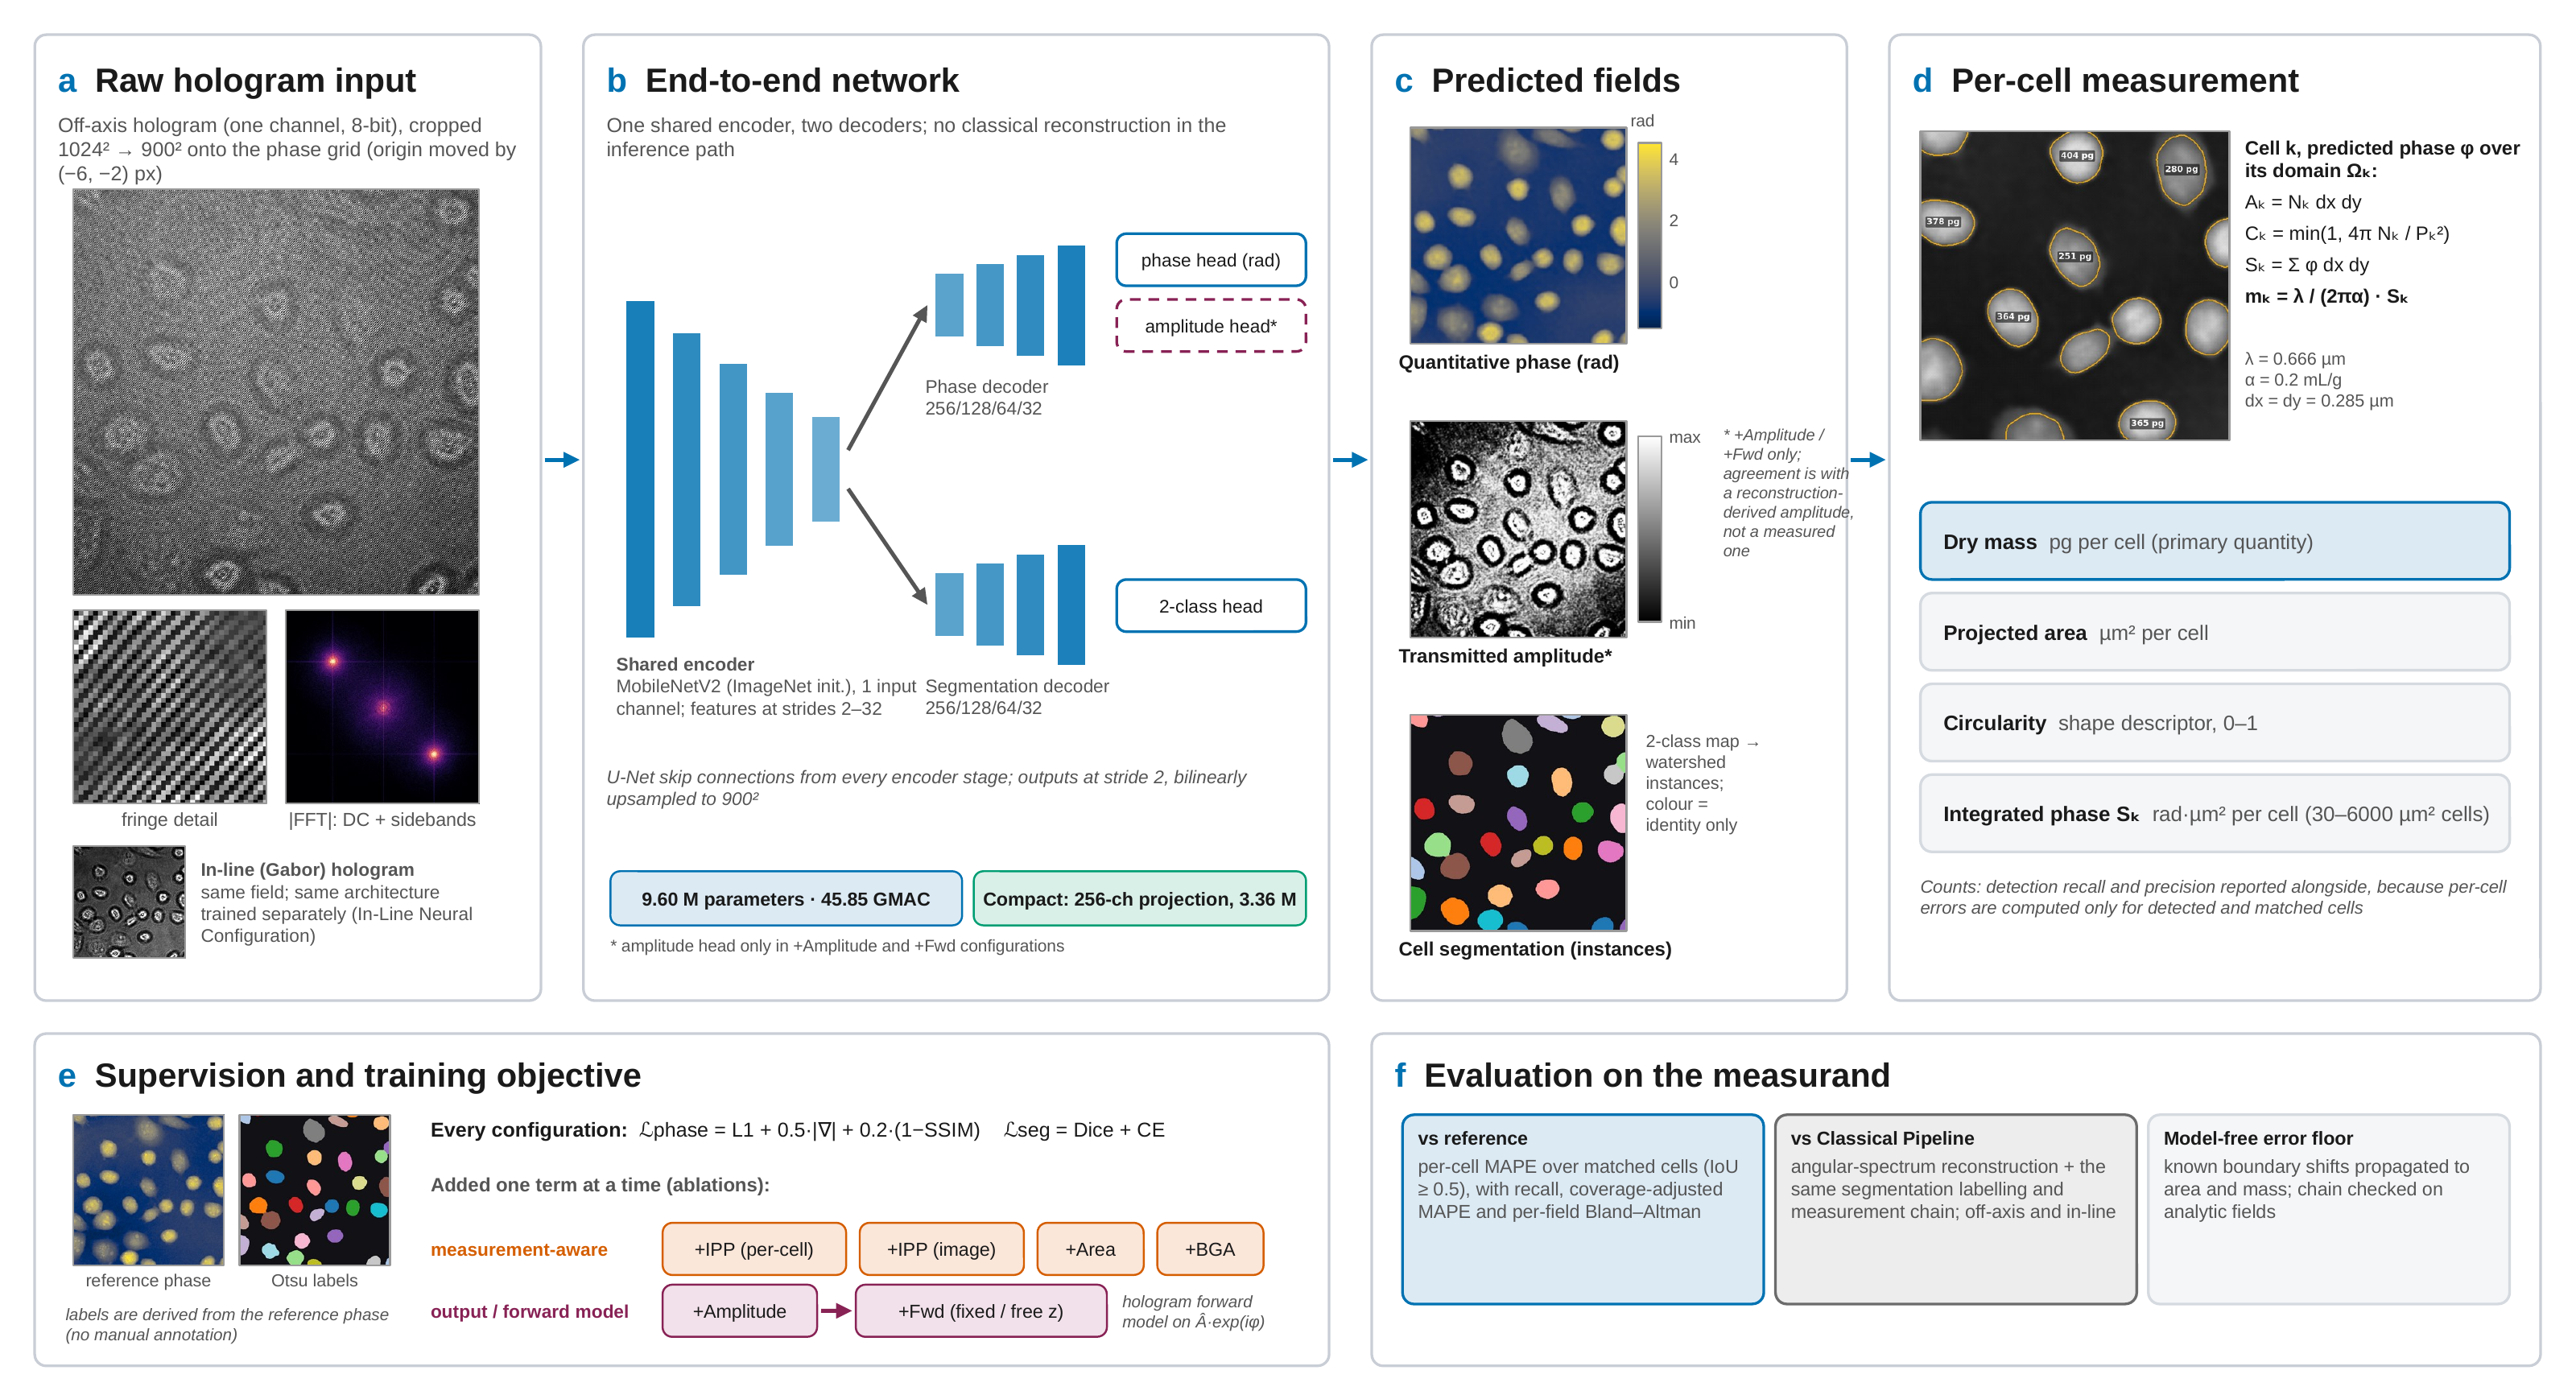
\includegraphics[width=\textwidth]{figure_1_overview.png}
\caption{Overview of the evaluated pipeline: (a) raw hologram input, cropped to
the phase grid; (b) network; (c) predicted outputs; (d) per-cell measurement;
(e) training configurations; (f) evaluation. Panels a, c and d show test field
NCI\_08; phase, segmentation and measurement are from the seed-42 End-to-End
Neural Baseline, and the amplitude map from +Amplitude.}
\label{fig:overview}
\end{figure}

\subsection{Hologram formation and propagation model}
\label{sec:formation}

A thin specimen illuminated by a plane wave transmits $U = A\,e^{i\varphi}$,
with $A$ the transmitted amplitude and $\varphi$ the phase. Propagation over a
distance $z$ is modelled with the angular-spectrum operator
\begin{equation}
\mathcal{P}_z\{U\} = \mathcal{F}^{-1}\!\left\{
\mathcal{F}\{U\}\,
e^{\,i 2\pi z \sqrt{\lambda^{-2}-f_x^2-f_y^2}}\right\},
\label{eq:angular-spectrum}
\end{equation}
with evanescent components attenuated as $e^{-2\pi|z|\sqrt{f_x^2+f_y^2-\lambda^{-2}}}$.
In the in-line (Gabor) geometry the sensor records
\begin{equation}
I_\mathrm{in} = \left|\mathcal{P}_z\{U\}\right|^2 ,
\label{eq:inline}
\end{equation}
which tends to $A^2$ as $z\rightarrow0$ and so carries phase only through
propagation. In the off-axis geometry a tilted reference $R$ is added,
\begin{equation}
I_\mathrm{off} = |R|^2 + |\mathcal{P}_z\{U\}|^2 + R^{*}\mathcal{P}_z\{U\} + R\,\mathcal{P}_z\{U\}^{*},
\label{eq:offaxis}
\end{equation}
and the object field appears in a carrier-modulated cross-term that can be
isolated in the Fourier plane at any $z$~\cite{cuche1999}. The classical
pipeline (Sec.~\ref{sec:classical}) and the forward-model term
(Sec.~\ref{sec:obj-fwd}) use these relations. The network itself receives only
the recorded intensity.

\subsection{Network architecture}
\label{sec:network}

A MobileNetV2 encoder~\cite{sandler2018mobilenetv2}, initialised from ImageNet
with its first convolution rebuilt for one input channel by averaging the RGB
filters, produces feature maps at strides 2--32. Two U-Net
decoders~\cite{ronneberger2015unet} with widths $256/128/64/32$ consume them: a
phase decoder that carries the phase head and, when enabled, the amplitude
head, and a segmentation decoder with a two-class head. The phase head has no
output activation and emits radians. The amplitude head outputs
$1 + 0.3\tanh(\cdot)$ and is zero-initialised, so it starts at unit
transmittance. The input is z-scored per field and reflection-padded to a
multiple of 32. The decoders end at stride 2, so the phase and segmentation maps
are produced at half resolution and bilinearly upsampled to $900\times900$. The
standard model has 9\,598\,099 parameters (45.85\,GMAC at $900\times900$). A
compact variant inserts a shared $1\times1$ projection from 1280 to 256 channels
before both decoders, which reduces the count to 3\,360\,403.

\subsection{Per-cell measurement domains and quantitative measurements}
\label{sec:measure}

Cell domains are the instances of a binary mask separated by a
distance-transform watershed (minimum peak distance 15\,px) and kept if their
area lies in 30--6000\,$\mu$m$^2$. The same instance labelling is applied to
predicted and reference masks. For each instance $\Omega_k$ with $N_k$ pixels
and Crofton perimeter $P_k$ (in pixels),
\begin{align}
A_k &= N_k\,dx\,dy , \label{eq:area}\\
C_k &= \min\!\left(1,\, 4\pi N_k / P_k^2\right) , \label{eq:circ}\\
S_k &= \textstyle\sum_{p\in\Omega_k}\varphi_p\,dx\,dy , \label{eq:volume}\\
m_k &= \frac{\lambda}{2\pi\alpha}\,S_k , \label{eq:mass}
\end{align}
with $dx=dy=0.284871\,\mu$m, $\lambda=0.666\,\mu$m and $\alpha=0.2$\,mL/g.
$S_k$ is the integrated phase in rad\,$\mu$m$^2$, and Eq.~\eqref{eq:mass} is the
dry-mass relation of~\cite{barer1952}. Circularity is evaluated on the pixel
grid, which is exact here because the sampling is isotropic. Predicted
measurements use the predicted phase inside predicted instances, and reference
measurements use the reference phase inside reference instances, with the same
code. Predicted and reference instances are paired one-to-one by greedy
descending IoU at IoU\,$\ge0.5$.

\subsection{Training objectives}
\label{sec:objective}

The objective is
\begin{equation}
\mathcal{L} = \Lphase + \Lseg
+ w_\mathrm{IPP}^\mathrm{cell}\Lippc + w_\mathrm{IPP}^\mathrm{img}\Lippi
+ w_\mathrm{area}\Larea
+ w_\mathrm{BGA}\Lbga
+ w_\mathrm{amp}\Lamp + w_\mathrm{fwd}\Lfwd ,
\label{eq:total}
\end{equation}
and every weight other than those of $\Lphase$ and $\Lseg$ is zero in the
baseline. The terms fall into two groups. The measurement-aware objectives
($\Lippc$, $\Lippi$, $\Larea$, $\Lbga$) encode the structure of the measurement
of Eq.~\eqref{eq:mass} and use no model of image formation. The forward-model
consistency term $\Lfwd$ is the only physics-based term: it compares the
prediction with the recorded hologram through Eqs.~\eqref{eq:angular-spectrum}
to~\eqref{eq:offaxis}.

\subsubsection{Supervised reconstruction and segmentation losses}
\label{sec:obj-sup}

The supervised terms are
\begin{align}
\Lphase &= \|\hat\varphi-\varphi\|_1
         + 0.5\,\bigl\||\nabla\hat\varphi|-|\nabla\varphi|\bigr\|_1
         + 0.2\,\bigl(1-\mathrm{SSIM}(\hat\varphi,\varphi)\bigr),
\label{eq:lphase}\\
\Lseg   &= \mathrm{Dice} + \mathrm{CE},\quad \text{class weights } (0.5, 1.0),
\label{eq:lseg}
\end{align}
with pixel-mean norms, forward-difference gradient magnitude, and SSIM over an
11-pixel Gaussian window ($\sigma=1.5$, data range 8\,rad).

\subsubsection{Measurement-aware objectives}
\label{sec:obj-mawo}

The measurement-aware terms couple the predicted phase to the predicted
foreground probability $f = 1 - p_\mathrm{background}$ from the segmentation
head. With $M$ the reference mask, $\Omega_k$ the reference instances of a
training crop, and $\epsilon = 10^{-4}$, the per-cell
integrated-phase-preservation (IPP) term is
\begin{equation}
\Lippc = \frac{1}{K}\sum_{k=1}^{K}
\frac{\left|\sum_{p\in\Omega_k} f_p\hat{\varphi}_p
           - \sum_{p\in\Omega_k} M_p\varphi_p\right|}
     {\left|\sum_{p\in\Omega_k} M_p\varphi_p\right| + \epsilon} ,
\label{eq:lipp}
\end{equation}
over the $K$ instances whose reference integral is at least 50\,rad\,px, with
each relative error capped at 10. The domains $\Omega_k$ are the watershed
instances of the reference mask, computed on the full field before cropping, so
an instance cut by a training crop is integrated over its visible part. Because
the domains are fixed reference instances, the term cannot be reduced by moving
them, and predicted foreground outside every reference instance does not enter
it. The image-level term replaces the per-cell sums with sums over the whole
crop,
\begin{equation}
\Lippi = \frac{\left|\sum_p f_p\hat{\varphi}_p - \sum_p M_p\varphi_p\right|}
            {\left|\sum_p M_p\varphi_p\right| + \epsilon} .
\label{eq:lpv}
\end{equation}
On a field with one cell over-measured by 20\% and another under-measured by
20\%, Eq.~\eqref{eq:lpv} is $0$ and Eq.~\eqref{eq:lipp} is $0.2$ (a unit test in
the repository). Since the quantity in Eq.~\eqref{eq:lipp} depends on both the
predicted foreground probability and the predicted phase inside $\Omega_k$, the
term can, as a formal property, be satisfied by a foreground that recedes inside
the reference domain together with a raised phase. The per-cell area term
constrains the domain directly,
\begin{equation}
\Larea = \frac{1}{K'}\sum_{k=1}^{K'}
\frac{\left|\sum_{p\in\Omega_k} f_p - \sum_{p\in\Omega_k} M_p\right|}
     {\sum_{p\in\Omega_k} M_p + \epsilon} ,
\label{eq:larea}
\end{equation}
over the $K'$ instances of at least 370\,px ($30\,\mu$m$^2$). It cannot penalise
foreground outside reference instances. The boundary--gradient alignment term
is
\begin{equation}
\Lbga = \left\|
\frac{|\nabla f|}{\max|\nabla f| + \epsilon'} -
\frac{|\nabla \hat\varphi|}{\max|\nabla \hat\varphi| + \epsilon'}
\right\|_1 ,\quad \epsilon'=10^{-8}.
\label{eq:lbga}
\end{equation}
These four terms are averaged over the crops of a batch that contain at least
370 reference-foreground pixels.

Measured before training over 30 batches of $512\times512$ crops, the gradient
of $\Lippc$ into the segmentation decoder at unit weight has a median magnitude
of $0.373$ (range $0.243$--$0.655$) times that of $\Lseg$ on the same
parameters. The central configuration uses $w_\mathrm{IPP}^\mathrm{cell}=1.0$,
and a sweep covers $0.1$, $0.3$, $1.0$ and $3.0$. $\Lippi$ is used at the same
coefficient, $w_\mathrm{IPP}^\mathrm{img}=1.0$; its gradient magnitude was not
matched to that of $\Lippc$.

\subsubsection{Amplitude objective}
\label{sec:obj-amp}

The amplitude term $\Lamp$ is the pixel-mean $\ell_1$ distance between the
predicted amplitude and the amplitude reference of Sec.~\ref{sec:labels}.

\subsubsection{Forward-model consistency}
\label{sec:obj-fwd}

$\Lfwd$ is the only term that compares the prediction with the recorded
hologram. The predicted field $\hat A\,e^{i(\hat\varphi+\Psi)}$ is
reflection-padded, propagated by Eq.~\eqref{eq:angular-spectrum}, and expanded
into the intensity components of Eq.~\eqref{eq:inline} or
Eq.~\eqref{eq:offaxis}. $\Psi$ is an order-5 polynomial aberration surface. It
is added back because the supplied phase had it removed while the recorded
hologram did not. A single surface, the per-coefficient median of per-field
fits over the training split, is used for every field, since per-field surfaces
are fitted against the reference phase and cannot be obtained at inference.
The unknown radiometric constants are removed by a per-image, ridge-regularised
least-squares fit of the recorded intensity $H$ onto the components $B_j$:
$\{1,|\mathcal{P}_z|^2\}$ in-line, and off-axis also the real and
imaginary parts of $R^{*}\mathcal{P}_z$ and $R\,\mathcal{P}_z$, with $R$ a plane
wave at the carrier frequency estimated from $H$. Carrying both conjugate
cross-terms and both quadratures makes the fit independent of which sideband is
selected and of the global piston phase $e^{i2\pi z/\lambda}$. With
$\hat H = \sum_j c_j B_j$ the fitted intensity,
\begin{equation}
\Lfwd = \frac{\sum_{p}\big(\hat H_p - H_p\big)^2}
             {\sum_{p}\big(H_p-\bar H\big)^2} ,
\label{eq:lfwd}
\end{equation}
evaluated after discarding a border of 79\,px (the diffraction spread at the
configured $z$). $\Lfwd$ is the fraction of the hologram's variance that the
synthesised hologram leaves unexplained. The propagation distance is fixed at
the supplied $z=33.77\,\mu$m or, in one configuration, made a trainable
parameter with its own learning rate ($100\times$ the base rate, no weight
decay). The pad and border stay fixed at the configured distance so that the
comparison domain does not change with $z$. Everything $\Lfwd$ uses is
available at inference: the carrier frequency and radiometric coefficients come
from the recorded hologram, and the global aberration surface from a one-time
calibration on training fields. A margin of $0.01$ in residual units is the
configured tolerance below which a difference in $\Lfwd$ is treated as noise
(Sec.~\ref{sec:res-fwd}).

% =============================================================================
\section{Experiments}
\label{sec:experiments}

\subsection{Dataset and imaging configuration}
\label{sec:data}

The dataset contains 800 fields of view of three human cancer cell lines
(NCI-H1299, SNU-475 and T-24; NCI, SNU and T24 below), each under a control
condition or one of four drugs: blebbistatin (myosin~II inhibition), FCCP
(mitochondrial uncoupling), staurosporine (apoptosis) and rotenone (complex~I
inhibition). Table~\ref{tab:dataset} gives the number of fields per cell line
and condition. The drug condition is a property of the dish, so it labels the
field, not the individual cell; it is not a network input or target and is used
only to stratify the split. Each field has an off-axis hologram and an in-line
Gabor hologram ($1024\times1024$, 8-bit), a $900\times900$ quantitative phase
map stored as float32 in radians, and a membrane-stain fluorescence image from a
separate camera. The illumination wavelength is $0.666\,\mu$m, the pixel pitch
at the sample $0.284871\,\mu$m, and the supplied propagation distance
$33.77\,\mu$m. The phase maps were supplied with the dataset as reconstructions
that are already aberration-corrected, background-subtracted and unwrapped; the
off-axis reconstruction principle is that of~\cite{cuche1999}, and we do not
know the exact processing chain that produced them. We use them as the phase
reference. Fields are split 560/127/113 (train/validation/test), stratified by
cell line $\times$ condition, and the same split is used for every off-axis
configuration and seed. The 113 test fields contain 3186 reference cells.
Acquisition, calibration and training settings are listed in
Table~\ref{tab:setup}.

% Table 1: dataset composition (fields per cell line and drug condition).
\begin{table}[!htbp]
\centering
\caption{Dataset composition: number of fields of view per cell line and drug
condition.}
\label{tab:dataset}
\footnotesize
\begin{tabular*}{\textwidth}{@{\extracolsep{\fill}}lrrrrrr@{}}
\toprule
Cell line & Ctrl & Bleb & FCCP & Stau & Rot & Total \\
\midrule
NCI   &  50 &  50 &  50 &  50 &  50 & 250 \\
SNU   & 100 &  50 &  50 &  50 &  50 & 300 \\
T24   &  50 &  50 &  50 &  50 &  50 & 250 \\
\midrule
Total & 200 & 150 & 150 & 150 & 150 & \textbf{800} \\
\bottomrule
\end{tabular*}
\tabnote{Ctrl, control; Bleb, blebbistatin; Stau, staurosporine; Rot, rotenone.}
\end{table}


The hologram is cropped from $1024$ to $900$\,px without resampling, with the
crop origin moved by $(-6, -2)$\,px in $(y, x)$ from the exactly centred crop.
The origin was determined by registering the classical off-axis reconstruction
(Sec.~\ref{sec:classical}) of each field to its reference phase. On the 127
validation fields, the centred crop left a median offset of $+5.4$\,px in $y$
and $+1.1$\,px in $x$. The rounded estimate and its eight neighbouring
whole-pixel origins were then evaluated on the same validation fields, and
$(-6,-2)$ gave median offsets of $0.0$ and $0.0$\,px. On the 113 test fields
the median residual offset at this origin is $-0.1$\,px in $y$ (5--95\%
range $-1.88$ to $+1.64$\,px) and $0.0$\,px in $x$ ($-3.06$ to $+2.12$\,px).
The same crop is used for the network input, the forward model, the
aberration fit, the amplitude reference and both classical pipelines.

The in-line holograms of fields SNU\_01 to SNU\_50 do not show the same field
of view as their off-axis holograms and reference phase. This was established
by registering each in-line frame to its off-axis hologram after band-pass
filtering (a Gaussian of $\sigma=5$\,px minus one of $\sigma=50$\,px, with a
Hann window), against a control in which every in-line frame was paired with a
different field's off-axis hologram by a random derangement. Matched pairs
were shifted by at most 1\,px on 734 of the 800 fields and control pairs on 3
of 800, and the correlation after registration separated matched from deranged
pairs with an AUC of $0.975$ ($0.973$ by registration error). The 750 correctly
paired fields all registered within 4.7\,px, 734 of them within 1\,px, with a
correlation after registration of $0.47$--$1.00$, above the highest control
value ($0.25$). The 50 fields SNU\_01 to SNU\_50 gave correlations of $-0.13$
to $0.18$, at the level of the unmatched control. A low-pass filter alone
($\sigma=5$\,px) did not separate matched from unmatched pairs (AUC $0.506$),
so the band-pass variant was used.
The off-axis holograms of these 50 fields do match the reference phase. They
were therefore excluded from the in-line modality only, before training, which
leaves an in-line split of 521/122/107 fields; every off-axis configuration
keeps all 800 fields. Comparisons across geometries use the 107 test fields
common to both (3055 reference cells).

% Table 2: acquisition, calibration, split and training settings.
\begin{table}[!htbp]
\centering
\caption{Acquisition, calibration, data split and training settings.}
\label{tab:setup}
\footnotesize
\begin{tabular*}{\textwidth}{@{\extracolsep{\fill}}ll@{}}
\toprule
\multicolumn{2}{@{}l}{\textbf{Acquisition and calibration}} \\
\midrule
Hologram                    & $1024\times1024$, 8-bit TIFF \\
Quantitative phase (reference) & $900\times900$, float32, radians \\
Hologram-to-phase mapping   & crop $1024\rightarrow900$, origin $(-6, -2)$\,px from the centred crop \\
Illumination wavelength $\lambda$ & $0.666\,\mu$m \\
Pixel pitch $dx=dy$         & $0.284871\,\mu$m \\
Refraction increment $\alpha$ & $0.2\,$mL/g \\
Propagation distance $z$    & $33.77\,\mu$m (supplied) \\
Aberration surface (forward model) & order-5 polynomial, median over training fields \\
\midrule
\multicolumn{2}{@{}l}{\textbf{Splits}} \\
\midrule
Off-axis fields (train / val / test) & 560 / 127 / 113 \\
In-line fields (train / val / test)  & 521 / 122 / 107 (SNU\_01--SNU\_50 excluded) \\
Stratification              & cell line $\times$ drug condition \\
Reference cells in test     & 3186 off-axis; 3055 in-line \\
\midrule
\multicolumn{2}{@{}l}{\textbf{Network}} \\
\midrule
Encoder                     & MobileNetV2, ImageNet-initialised \\
Decoders                    & two U-Net decoders, 256/128/64/32 \\
Heads                       & phase, amplitude (optional), segmentation (2 classes) \\
Network input               & raw hologram, z-scored per field \\
Output grid                 & stride 2, bilinearly upsampled \\
Parameters, standard        & 9\,598\,099 (45.85\,GMAC) \\
Parameters, with amplitude  & 9\,607\,412 (47.87\,GMAC) \\
Parameters, compact         & 3\,360\,403 (24.03\,GMAC) \\
\midrule
\multicolumn{2}{@{}l}{\textbf{Optimisation}} \\
\midrule
Epochs                      & 60 \\
Optimiser                   & AdamW, $\beta=(0.9,0.999)$ \\
Learning rate               & $3\times10^{-4}$, 2 warm-up epochs, cosine to $10^{-6}$ \\
Learning rate for $z$ (+Fwd, free $z$)& $100\times$ base \\
Weight decay                & $1\times10^{-4}$ \\
Batch size / train crop     & 4 / $512\times512$ \\
Precision                   & mixed, FP16 \\
Gradient clipping           & 1.0 (global norm) \\
Augmentation                & flips, $90^\circ$ rotations \\
Checkpoint criterion        & best validation composite (Sec.~\ref{sec:stats}), every epoch, no early stopping \\
Seeds                       & 42 (primary), 1337, 2024 \\
\bottomrule
\end{tabular*}
\end{table}


\subsection{Reference phase, segmentation labels and amplitude reference}
\label{sec:labels}

No manual annotation is available, so the reference masks are derived from the
reference phase: Gaussian smoothing ($\sigma=4$\,px), a per-field Otsu
threshold, binary closing (2\,px), hole filling, removal of objects touching the
array border, and the area filter of Sec.~\ref{sec:measure}. Instances are
separated with the watershed of Sec.~\ref{sec:measure}. These are
phase-derived, silver-standard labels: the segmentation target is a
deterministic function of the phase target. Two further properties of the
construction matter for the results. The closing step leaves an empty
two-pixel rim at the array border, so the border-removal step, as configured,
removes no objects, and objects truncated by the field edge and elongated
regions along the field boundary remain in the reference
(Fig.~\ref{fig:qualitative}; quantified in Sec.~\ref{sec:res-measure}). The
Otsu level also varies across fields ($0.406 \pm 0.151$\,rad over 800 fields)
and differs between drug conditions (one-way ANOVA $F=15.26$,
$p=4.9\times10^{-12}$).

As a check that does not depend on the phase, the membrane channel was
registered to the phase grid (scale $1.343769$, equal to the ratio of the
phase pixel pitch, $0.284871\,\mu$m, to the second pitch value stored in the
phase-file header, $0.211994\,\mu$m, which the registration search also
preferred on all 13 fields tested; fitted offset $314/280$\,px in $y/x$ on the
phase grid), Gaussian-smoothed ($\sigma=2$\,px), thresholded at the 75th
percentile of the illuminated region, opened with a $3\times3$ structuring
element and hole-filled. The stain marks cell perimeters, so these masks are
provisional. They are used only in Sec.~\ref{sec:res-measure}.

No measured amplitude exists for these data. For the configurations with an
amplitude output, the target is the modulus of a classical off-axis
reconstruction (first-order sideband isolation) of the cropped hologram,
normalised to a background median of 1 and clipped at 1.5. It is a
reconstruction-derived reference, not ground truth.

\subsection{Training and experimental configurations}
\label{sec:arms}

Table~\ref{tab:arms} lists the configurations. Each differs from its comparator
by one term, one output or one capacity choice. The End-to-End Neural Baseline
uses $\Lphase+\Lseg$ on off-axis holograms, and the In-Line Neural
Configuration applies the same objective to the in-line holograms of the 750
correctly paired fields; the two geometries are trained separately and share no
weights. +IPP (per-cell) and +IPP (image) each add one integrated-phase term to
the baseline at the same coefficient, $w=1.0$, so their comparison is an
equal-coefficient comparison in which the gradient magnitudes were not matched.
+Area and +BGA each add one term to +IPP (per-cell). +Amplitude adds the
amplitude head and $\Lamp$ ($w=0.1$) to +IPP (per-cell). +Fwd (fixed $z$) adds
$\Lfwd$ ($w=0.02$) to +Amplitude, because the term uses the predicted complex
field, and +Fwd (free $z$) makes $z$ trainable. The Compact Baseline and
Compact +IPP are the baseline and +IPP (per-cell) with the compact decoder. All
configurations are off-axis except the In-Line Neural Configuration. The $w=1.0$
member of the weight sweep is +IPP (per-cell) itself. Training settings are in
Table~\ref{tab:setup}.

% Table 3: experimental configurations and the single change each makes.
\begin{table}[!htbp]
\centering
\caption{Experimental configurations. Each differs from its comparator by one
change; weights not listed are zero. Seeds: number of training runs.}
\label{tab:arms}
\footnotesize
\begin{tabularx}{\textwidth}{@{}>{\raggedright\arraybackslash}p{3.6cm}>{\raggedright\arraybackslash}X>{\raggedright\arraybackslash}p{3.6cm}c@{}}
\toprule
Configuration & Change relative to comparator & Comparator & Seeds \\
\midrule
\multicolumn{4}{@{}l}{\emph{Main pipeline and hologram mode}} \\
End-to-End Neural Baseline & off-axis; reconstruction + segmentation losses only & -- & 3 \\
In-Line Neural Configuration & the baseline's objective on in-line Gabor holograms; SNU\_01--SNU\_50 excluded & End-to-End Neural Baseline & 1 \\
\midrule
\multicolumn{4}{@{}l}{\emph{Measurement-aware objectives}} \\
+IPP (per-cell) & $+\,\mathcal{L}_\mathrm{IPP}^\mathrm{cell}$, $w=1.0$ & End-to-End Neural Baseline & 3 \\
+IPP (image) & $+\,\mathcal{L}_\mathrm{IPP}^\mathrm{img}$, $w=1.0$ & End-to-End Neural Baseline & 3 \\
+Area & $+\,\mathcal{L}_\mathrm{area}$, per-cell, $w=1.0$ & +IPP (per-cell) & 1 \\
+BGA & $+\,\mathcal{L}_\mathrm{BGA}$, $w=0.05$ & +IPP (per-cell) & 1 \\
+IPP (per-cell), $w=0.1/0.3/3.0$ & $\mathcal{L}_\mathrm{IPP}^\mathrm{cell}$ weight $0.1$, $0.3$, $3.0$ & End-to-End Neural Baseline & 1 \\
\midrule
\multicolumn{4}{@{}l}{\emph{Amplitude output and forward-model consistency}} \\
+Amplitude & $+$ amplitude head, $+\,\mathcal{L}_\mathrm{amp}$, $w=0.1$ & +IPP (per-cell) & 1 \\
+Fwd (fixed $z$) & $+\,\mathcal{L}_\mathrm{fwd}$, $w=0.02$, $z$ fixed & +Amplitude & 1 \\
+Fwd (free $z$) & $z$ becomes a trainable parameter & +Fwd (fixed $z$) & 1 \\
\midrule
\multicolumn{4}{@{}l}{\emph{Model capacity}} \\
Compact Baseline & shared $1\times1$ projection to 256 channels before the decoders (3.36\,M parameters) & End-to-End Neural Baseline & 1 \\
Compact +IPP & compact decoder, with $\mathcal{L}_\mathrm{IPP}^\mathrm{cell}$ & +IPP (per-cell) & 1 \\
\bottomrule
\end{tabularx}
\end{table}


\subsection{Classical comparison pipeline}
\label{sec:classical}

The comparison is with one classical configuration per geometry, scored by the
same instance labelling and measurement code. Off-axis, it is first-order
sideband isolation (radius 130\,px, DC exclusion 60\,px), conjugate-sideband
selection by phase skewness, and angular-spectrum back-propagation to
$33.77\,\mu$m. In-line, it is back-propagation of the recorded amplitude
($\sqrt{I}$) to $33.77\,\mu$m followed by 20 Gerchberg--Saxton iterations with
the sample-plane modulus constrained to at most 1. Both are followed by phase
unwrapping, subtraction of an order-3 polynomial fitted to background pixels of
a preliminary mask, and the reference-mask rule of Sec.~\ref{sec:labels}
applied to the resulting phase. The classical segmentation is thus the
labelling rule itself applied to a classical reconstruction. Both pipelines use
the crop of Sec.~\ref{sec:data}.

\subsection{Evaluation protocol}
\label{sec:eval}

All metrics are computed at full $900\times900$ resolution, on the 113
off-axis test fields unless stated, and the cross-geometry comparison on the
107 common test fields.

\emph{Reconstruction.} Phase MAE over the field and inside reference cells,
Pearson $r$ and SSIM between predicted and reference phase describe the phase
map, an intermediate output.

\emph{Segmentation and detection.} Dice, AJI and boundary F1 at 2\,px
tolerance describe the mask, also an intermediate output. Detection recall and
precision are computed from the IoU matching of Sec.~\ref{sec:measure}.

\emph{Per-cell measurement.} Mean absolute percentage error (MAPE) and per-cell
Pearson $r$ of projected area, circularity and dry mass are computed over
matched cells only, so they describe how well detected cells are measured.
Because $\lambda/(2\pi\alpha)$ multiplies predicted and reference $S_k$ alike,
the relative error of the integrated phase of a cell equals its relative
dry-mass error, and every relative error, correlation and relative bias of dry
mass reported here is independent of $\lambda$ and $\alpha$. We report it once,
as dry-mass MAPE.

\emph{Coverage and field totals.} Matched-cell errors are reported beside
recall and a coverage-adjusted error that charges each missed reference cell as
a 100\% error,
\begin{equation}
\mathrm{MAPE}_\mathrm{cov} = r_\mathrm{det}\cdot\mathrm{MAPE} + (1-r_\mathrm{det}) ,
\label{eq:covadj}
\end{equation}
and beside field totals, which sum all predicted and all reference cells on a
field without pairing; their error is reported as a field-total MAPE and a
field-total bias. Method agreement is reported as a relative Bland--Altman
analysis~\cite{blandaltman1986} on per-field medians of matched cells.

\emph{Mass-error decomposition.} With $S(\Omega,\varphi)=\sum_{p\in\Omega}
\varphi_p\,dx\,dy$, the ratio of predicted to reference dry mass factorises
exactly,
\begin{equation}
\frac{\hat m}{m} =
\underbrace{\frac{S(\hat\Omega,\varphi)}{S(\Omega,\varphi)}}_{\text{domain factor}}
\times
\underbrace{\frac{S(\hat\Omega,\hat\varphi)}{S(\hat\Omega,\varphi)}}_{\text{phase factor}} ,
\label{eq:decomp}
\end{equation}
where $\hat\Omega$ and $\Omega$ are the predicted and reference domains. The
domain factor holds the phase at the reference and changes only the domain; the
phase factor holds the domain at the prediction and changes only the phase. At
cell level, $\Omega$ is a reference instance and $\hat\Omega$ the predicted
instance matched to it, and cells are split into edge cells (a reference pixel
within 3\,px of the field boundary) and interior cells. At field level,
$\hat\Omega$ and $\Omega$ are the whole predicted and reference foreground, so
undetected and spurious cells enter the domain factor. Each factor is
summarised by its geometric mean, which composes exactly, and by the median
absolute log ratio as a sign-free measure of spread. The decomposition
describes how the error is structured; it does not identify what causes it.

\subsection{Computational benchmarking protocol}
\label{sec:bench-protocol}

Inference cost was measured at $900\times900$ and batch 1 on one NVIDIA
RTX~A5000, in PyTorch~2.6 and in ONNX Runtime (opset 17, CUDA execution
provider); the FP16 models are half-precision exports of weights and input.
Each measurement is 50 warm-up passes followed by 500 timed passes. The
baseline was benchmarked once per trained seed, every other configuration once.
The $p_{99}/p_{50}$ latency ratio is recorded as a check on timing stability,
with a limit of 1.25. Weight size and peak allocated memory are reported for
PyTorch only, because ONNX Runtime does not expose comparable allocator
accounting; the peak allocation does not separate this process's CUDA context
from other jobs on the device.

\subsection{Model-free sensitivity analyses}
\label{sec:modelfree}

Boundary sensitivity is measured on the off-axis test fields by dilating or
eroding each reference instance by 1--5 pixels and recomputing area and dry
mass from the reference phase. The numerical error of the measurement chain is
measured on synthetic fields of spherical-cap cells,
$\varphi(d)=\varphi_0\sqrt{1-(d/r)^2}$, whose area $\pi r^2$ and integrated
phase $\tfrac{2}{3}\pi r^2\varphi_0$ are exact. Three independently generated
sets are used.

\subsection{Statistical analysis}
\label{sec:stats}

The baseline, +IPP (per-cell) and +IPP (image) were trained at seeds 42, 1337
and 2024, and every other configuration once, at seed 42. Values reported for
the replicated configurations are three-run means with the between-seed sample
SD. A difference between two configurations is called \emph{resolved} if it
exceeds twice the pooled between-seed standard deviation,
$2\sqrt{(s_1^2+s_2^2)/2}$, of the same metric. This is a separation criterion
defined before the comparisons were made; no hypothesis test is performed, and a
comparison in which either configuration has fewer than three runs is reported
as not resolvable. Within-run intervals are percentile bootstrap intervals over
fields (2000 resamples). Evaluation is deterministic in data and weights but
not bit-exact, because convolution algorithms are selected at run time.
Checkpoints were selected on the validation split by
$0.35\,\mathrm{Dice}+0.25\,r_\varphi+0.25\,(1-\mathrm{MAPE}_\mathrm{mass})+0.15\,F1_\mathrm{det}$,
so the validation dry-mass error enters model selection but not training.
Location stratification (edge and interior) and the mass-error decomposition
were computed after training, from the stored models and reference masks.

% =============================================================================
\section{Results}
\label{sec:results}

\subsection{Reconstruction and segmentation from raw holograms}
\label{sec:res-recon}

On the 113 off-axis test fields, the End-to-End Neural Baseline has, compared
with the tested classical pipeline, lower phase error (MAE
$0.1968\rightarrow0.1568$\,rad; inside reference cells
$0.3112\rightarrow0.2689$\,rad), higher phase correlation
($0.7851\rightarrow0.8741$) and higher SSIM ($0.5299\rightarrow0.6386$)
(Table~\ref{tab:learned-vs-classical}, Fig.~\ref{fig:learned-vs-classical}a).
The segmentation scores are closer: Dice $0.8253\rightarrow0.8337$, AJI
$0.6387\rightarrow0.6710$ and boundary F1 $0.3954\rightarrow0.4687$, a relative
increase of 19\%. Recall is nearly the same ($0.5869$ and $0.5931$) and
precision is higher for the network ($0.7910\rightarrow0.8488$). At the
measurement level, projected-area MAPE is essentially equal ($0.1578$ and
$0.1568$) while the matched-cell dry-mass MAPE is lower for the network
($0.2203\rightarrow0.1742$), with a per-cell dry-mass correlation of $0.9363$
against $0.8937$. The field-total dry-mass MAPE goes the other way: $0.1094$ for
the tested classical pipeline and $0.1631\pm0.0141$ for the network
(Sec.~\ref{sec:res-measure}). All comparisons in this paragraph are with the
tested classical pipeline only.

% Table 4: End-to-End Neural Baseline against the tested classical pipeline, off-axis, 113 test fields.
\begin{table}[!htbp]
\centering
\caption{End-to-End Neural Baseline and the tested classical pipeline on the
off-axis test set (113 fields, 3186 reference cells). Neural values are mean
$\pm$ SD over three training seeds; the classical pipeline is deterministic and
was run once. $\Delta$: neural minus classical.}
\label{tab:learned-vs-classical}
\footnotesize
\begin{tabular*}{\textwidth}{@{\extracolsep{\fill}}lrrr@{}}
\toprule
Quantity & Classical & Neural ($n=3$) & $\Delta$ \\
\midrule
Phase MAE [rad] $\downarrow$ & 0.1968 & $0.1568 \pm 0.0023$ & $-0.0400$ \\
Phase MAE inside cells [rad] $\downarrow$ & 0.3112 & $0.2689 \pm 0.0056$ & $-0.0423$ \\
Phase Pearson $r$ $\uparrow$ & 0.7851 & $0.8741 \pm 0.0023$ & $+0.0890$ \\
Phase SSIM $\uparrow$ & 0.5299 & $0.6386 \pm 0.0053$ & $+0.1087$ \\
\midrule
Dice $\uparrow$ & 0.8253 & $0.8337 \pm 0.0013$ & $+0.0085$ \\
AJI $\uparrow$ & 0.6387 & $0.6710 \pm 0.0025$ & $+0.0322$ \\
Boundary F1 $\uparrow$ & 0.3954 & $0.4687 \pm 0.0053$ & $+0.0733$ \\
Detection recall $\uparrow$ & 0.5869 & $0.5931 \pm 0.0027$ & $+0.0062$ \\
Detection precision $\uparrow$ & 0.7910 & $0.8488 \pm 0.0124$ & $+0.0577$ \\
\midrule
Projected-area MAPE $\downarrow$ & 0.1578 & $0.1568 \pm 0.0027$ & $-0.0010$ \\
Dry-mass MAPE $\downarrow$ & 0.2203 & $0.1742 \pm 0.0045$ & $-0.0461$ \\
Dry-mass Pearson $r$, per cell $\uparrow$ & 0.8937 & $0.9363 \pm 0.0007$ & $+0.0427$ \\
Field-total dry-mass MAPE $\downarrow$ & 0.1094 & $0.1631 \pm 0.0141$ & $+0.0537$ \\
Cells matched (of 3186) & 1870 & $1890 \pm 9$ & $+20 \pm 9^{\dagger}$ \\
\bottomrule
\end{tabular*}
\tabnote{$^{\dagger}$Descriptive difference of the matched-cell count (neural mean minus classical; the SD is the between-seed SD of the neural count). A matched-cell count is not an error metric, and the resolution criterion of Sec.~\ref{sec:stats} is not applied to it. The classical pipeline is deterministic, so no difference in this table is assessed against a between-seed spread.}
\end{table}


\begin{figure}[!htbp]
\centering
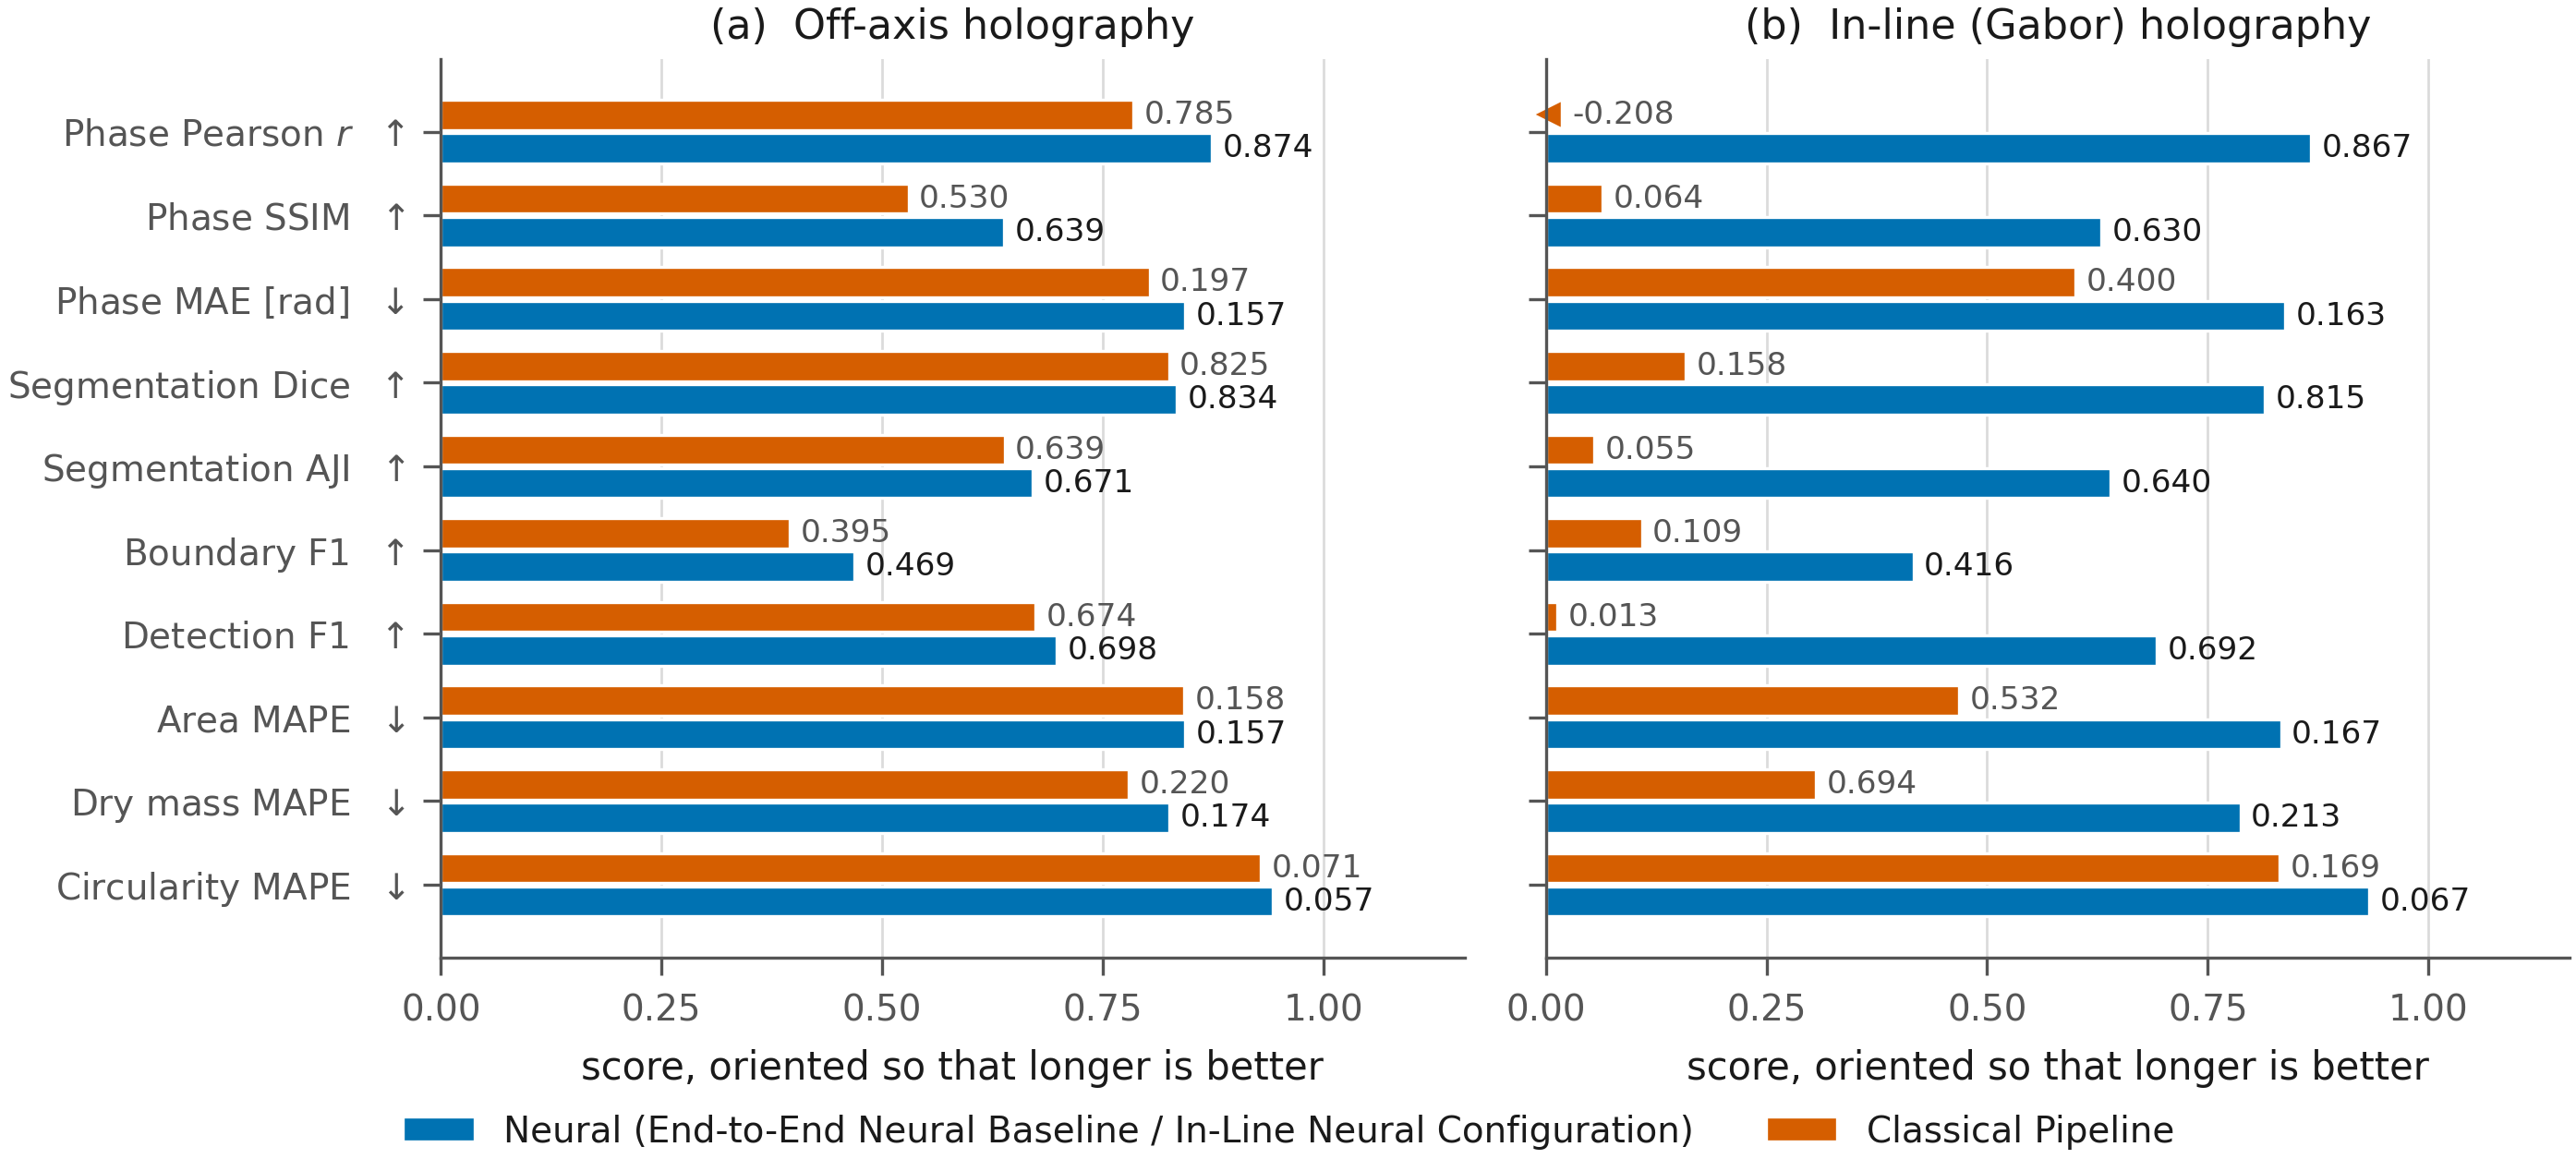
\includegraphics[width=\textwidth]{figure_2.png}
\caption{Neural and tested classical pipelines, oriented so that longer bars are
better (error metrics drawn as $1-$error, raw value printed). (a) Off-axis, 113
test fields; End-to-End Neural Baseline, mean over three seeds. (b) In-line, the
107 correctly paired test fields; In-Line Neural Configuration, one run. The
negative phase correlation of the classical in-line reconstruction is drawn at
zero with a left-pointing marker.}
\label{fig:learned-vs-classical}
\end{figure}

Table~\ref{tab:common} compares the two geometries on the 107 test fields whose
in-line hologram is correctly paired. The In-Line Neural Configuration reaches
phase $r=0.8667$, Dice $0.8148$, boundary F1 $0.4165$, recall $0.5885$ and a
dry-mass MAPE of $0.2129$ over 1798 matched cells. On the same fields the
off-axis baseline has phase $r=0.8745\pm0.0023$, Dice $0.8330\pm0.0013$,
boundary F1 $0.4706\pm0.0052$, recall $0.5936\pm0.0031$ and dry-mass MAPE
$0.1740\pm0.0045$. The in-line configuration was trained once, so these
differences (for example $+0.0389$ in dry-mass MAPE) are not resolvable under
our criterion. The tested classical in-line reconstruction did not recover the
specimen phase ($r=-0.2075$), consistent with the behaviour reported for a
500-iteration Gerchberg--Saxton reconstruction in Park
\emph{et al.}~\cite{park2026ai} (Supplementary Section~S2), whose phase profile
remained near the background.
Our in-line reconstruction used 20 iterations at $33.77\,\mu$m. Its in-cell
phase contrast (median over the 107 fields of the mean phase inside the reference
cells minus the mean outside, computed identically for all columns of
Table~\ref{tab:common}) is $-0.084$\,rad, against $+0.922$\,rad for the
classical off-axis reconstruction on the same fields; the reference phase gives
$+1.097$\,rad, the In-Line Neural Configuration $+0.887$\,rad and the off-axis
baseline $+0.899\pm0.036$\,rad. The classical in-line pipeline matched 106 of
3055 reference cells (Dice $0.1583$). Its measurements are therefore computed
from a phase map that does not carry the specimen contrast, and its per-cell
dry-mass correlation, over 106 cells, is not comparable with the other
entries. This result concerns the tested in-line configuration and does not
describe classical in-line reconstruction in general.

% Table 5: both geometries on the 107 test fields whose in-line hologram is correctly paired.
\begin{table}[!htbp]
\centering
\caption{Off-axis and in-line pipelines on the 107 test fields common to both
geometries (3055 reference cells; SNU\_01--SNU\_50 excluded). In-line neural:
one training run; off-axis neural: mean $\pm$ SD over three seeds, the same
models as in Table~\ref{tab:learned-vs-classical} re-scored on these fields;
classical pipelines: one deterministic run each. $n$: number of training runs.}
\label{tab:common}
\footnotesize
\begin{tabular*}{\textwidth}{@{\extracolsep{\fill}}lrrrr@{}}
\toprule
 & \multicolumn{2}{c}{Neural} & \multicolumn{2}{c}{Classical} \\
\cmidrule(lr){2-3}\cmidrule(lr){4-5}
Quantity & In-line ($n=1$) & Off-axis ($n=3$) & Off-axis & In-line \\
\midrule
Recovered in-cell phase contrast [rad]$^{\ddagger}$ & $+0.887$ & $+0.899 \pm 0.036$ & $+0.922$ & $-0.084$ \\
\midrule
Phase MAE [rad] $\downarrow$ & 0.1625 & $0.1586 \pm 0.0024$ & 0.1990 & 0.3996 \\
Phase MAE inside cells [rad] $\downarrow$ & 0.3005 & $0.2726 \pm 0.0057$ & 0.3157 & 1.0448 \\
Phase Pearson $r$ $\uparrow$ & 0.8667 & $0.8745 \pm 0.0023$ & 0.7849 & $-0.2075$ \\
Phase SSIM $\uparrow$ & 0.6296 & $0.6377 \pm 0.0053$ & 0.5297 & 0.0639 \\
\midrule
Dice $\uparrow$ & 0.8148 & $0.8330 \pm 0.0013$ & 0.8240 & 0.1583 \\
AJI $\uparrow$ & 0.6399 & $0.6697 \pm 0.0031$ & 0.6355 & 0.0549 \\
Boundary F1 $\uparrow$ & 0.4165 & $0.4706 \pm 0.0052$ & 0.3943 & 0.1087 \\
Detection recall $\uparrow$ & 0.5885 & $0.5936 \pm 0.0031$ & 0.5849 & 0.0347 \\
Detection precision $\uparrow$ & 0.8406 & $0.8487 \pm 0.0140$ & 0.7883 & 0.0077 \\
\midrule
Projected-area MAPE $\downarrow$ & 0.1669 & $0.1552 \pm 0.0025$ & 0.1576 & 0.5315 \\
Dry-mass MAPE $\downarrow$ & 0.2129 & $0.1740 \pm 0.0045$ & 0.2204 & 0.6942 \\
Field-total dry-mass MAPE $\downarrow$ & 0.1356 & $0.1657 \pm 0.0145$ & 0.1101 & 0.6602 \\
\midrule
Dry-mass Pearson $r$, per cell $\uparrow$ & 0.9029 & $0.9374 \pm 0.0010$ & 0.8940 & 0.8758$^{\ast}$ \\
Cells matched (of 3055) & 1798 & $1813 \pm 10$ & 1787 & 106 \\
\bottomrule
\end{tabular*}
\tabnote{$^{\ast}$Computed over the 106 cells matched by the classical in-line pipeline; not comparable with the other columns. $^{\ddagger}$Median over the 107 fields of the mean phase inside the reference cell masks minus the mean phase outside them, computed identically for all four columns; the reference phase gives $+1.097$\,rad. The differences between the single in-line run and the three off-axis runs are not resolvable under the criterion of Sec.~\ref{sec:stats}.}
\end{table}


Figure~\ref{fig:qualitative} shows the seed-42 baseline on the first two test
fields of the split, NCI\_06 and NCI\_08, without selection. The signed phase
error is small over most of the background and largest in bands along the field
edges, and the reference masks include regions along the field boundary that
the network does not segment.

\begin{figure}[!htbp]
\centering
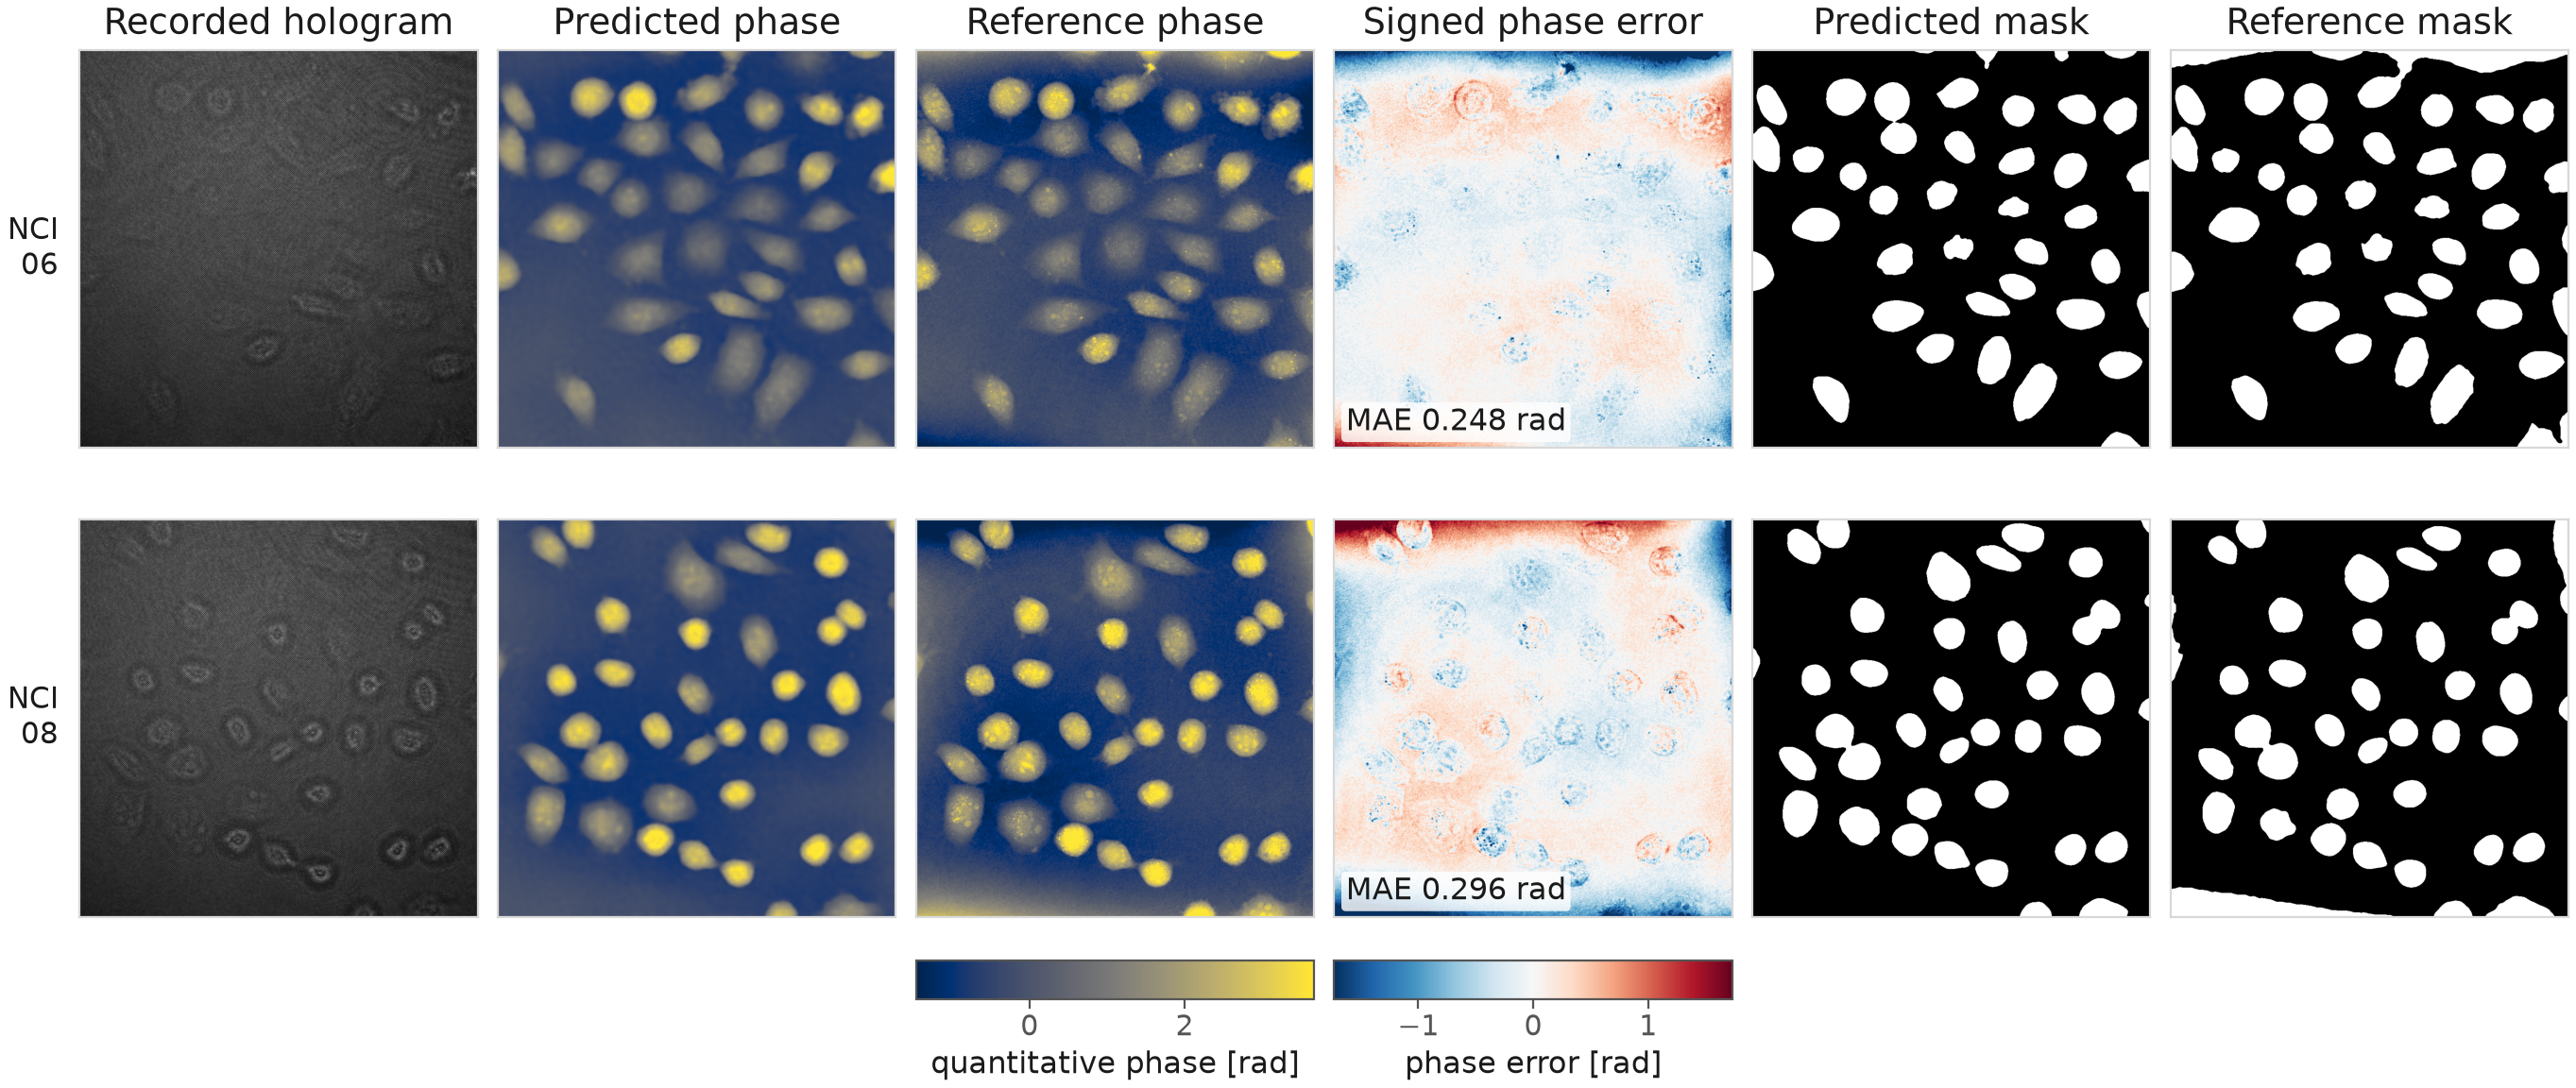
\includegraphics[width=\textwidth]{figure_3.png}
\caption{Outputs of the seed-42 End-to-End Neural Baseline on test fields
NCI\_06 (top) and NCI\_08 (bottom): recorded off-axis hologram (cropped to the
phase grid), predicted and reference phase on a shared colour scale, signed
phase error (prediction minus reference, field MAE printed), and predicted and
reference masks.}
\label{fig:qualitative}
\end{figure}

\subsection{Per-cell measurements, error decomposition and population coverage}
\label{sec:res-measure}

Over $1890\pm9$ matched cells (mean over three seeds; the seed-42 run shown in
Fig.~\ref{fig:agreement} has 1898), the baseline's per-cell dry-mass MAPE is
$0.1742\pm0.0045$ (seed-42 bootstrap interval $0.1650$--$0.1849$) with a
per-cell Pearson $r$ of $0.9363$. Projected area has MAPE $0.1568$ and
$r=0.8986$, and circularity has MAPE $0.0571$ and $r=0.8861$
(Table~\ref{tab:measurement}a). The per-field Bland--Altman bias, computed on
per-field medians and averaged over seeds, is $-0.0372$ for dry mass (limits
$[-0.247,+0.172]$) and $+0.0649$ for projected area ($[-0.162,+0.292]$), so on
matched cells area is slightly over-estimated and dry mass under-estimated
(Table~\ref{tab:measurement}b, Fig.~\ref{fig:agreement}). Field totals, which
include unmatched cells on both sides, are low for both quantities
($-0.0901$ area, $-0.1560$ dry mass), with a field-total dry-mass correlation of
$0.9883$.

% Table 6: per-cell and per-field measurement agreement of the End-to-End Neural Baseline.
\begin{table}[!htbp]
\centering
\caption{Measurement agreement of the End-to-End Neural Baseline on the
off-axis test set (113 fields, 3186 reference cells). Mean $\pm$ SD over three
training seeds unless stated. (a) Matched cells. (b) Relative Bland--Altman
statistics on per-field medians of matched cells, and field totals over all
predicted and all reference cells.}
\label{tab:measurement}
\footnotesize
\textbf{(a) Matched cells}\\[2pt]
\begin{tabular*}{\textwidth}{@{\extracolsep{\fill}}lcccc@{}}
\toprule
Quantity & MAPE & 95\% CI (seed 42) & Cov.-adj. MAPE & Pearson $r$ \\
\midrule
Projected area & $0.1568 \pm 0.0027$ & 0.1471--0.1663 & $0.4999 \pm 0.0036$ & $0.8986 \pm 0.0011$ \\
Circularity & $0.0571 \pm 0.0027$ & 0.0493--0.0633 & $0.4408 \pm 0.0039$ & $0.8861 \pm 0.0072$ \\
Dry mass & $0.1742 \pm 0.0045$ & 0.1650--0.1849 & $0.5102 \pm 0.0041$ & $0.9363 \pm 0.0007$ \\
\bottomrule
\end{tabular*}

\vspace{8pt}
\textbf{(b) Per field and field totals}\\[2pt]
\begin{tabular*}{\textwidth}{@{\extracolsep{\fill}}lccccc@{}}
\toprule
 & \multicolumn{2}{c}{Bland--Altman (per field)} & \multicolumn{3}{c}{Field total} \\
\cmidrule(lr){2-3}\cmidrule(lr){4-6}
Quantity & Bias & Limits of agreement & Bias & MAPE & Pearson $r$ \\
\midrule
Projected area & $+0.0649 \pm 0.0028$ & $[-0.162, +0.292]$ & $-0.0901 \pm 0.0037$ & $0.1553 \pm 0.0047$ & $0.9341 \pm 0.0043$ \\
Circularity & $+0.0217 \pm 0.0057$ & $[-0.054, +0.097]$ & -- & -- & -- \\
Dry mass & $-0.0372 \pm 0.0172$ & $[-0.247, +0.172]$ & $-0.1560 \pm 0.0174$ & $0.1631 \pm 0.0141$ & $0.9883 \pm 0.0007$ \\
\bottomrule
\end{tabular*}
\tabnote{CI: percentile bootstrap over fields (2000 resamples) of the seed-42
run. Limits of agreement: means over seeds. Dry mass and integrated phase $S_k$
have identical relative statistics (Sec.~\ref{sec:eval}).}
\end{table}


\begin{figure}[!htbp]
\centering
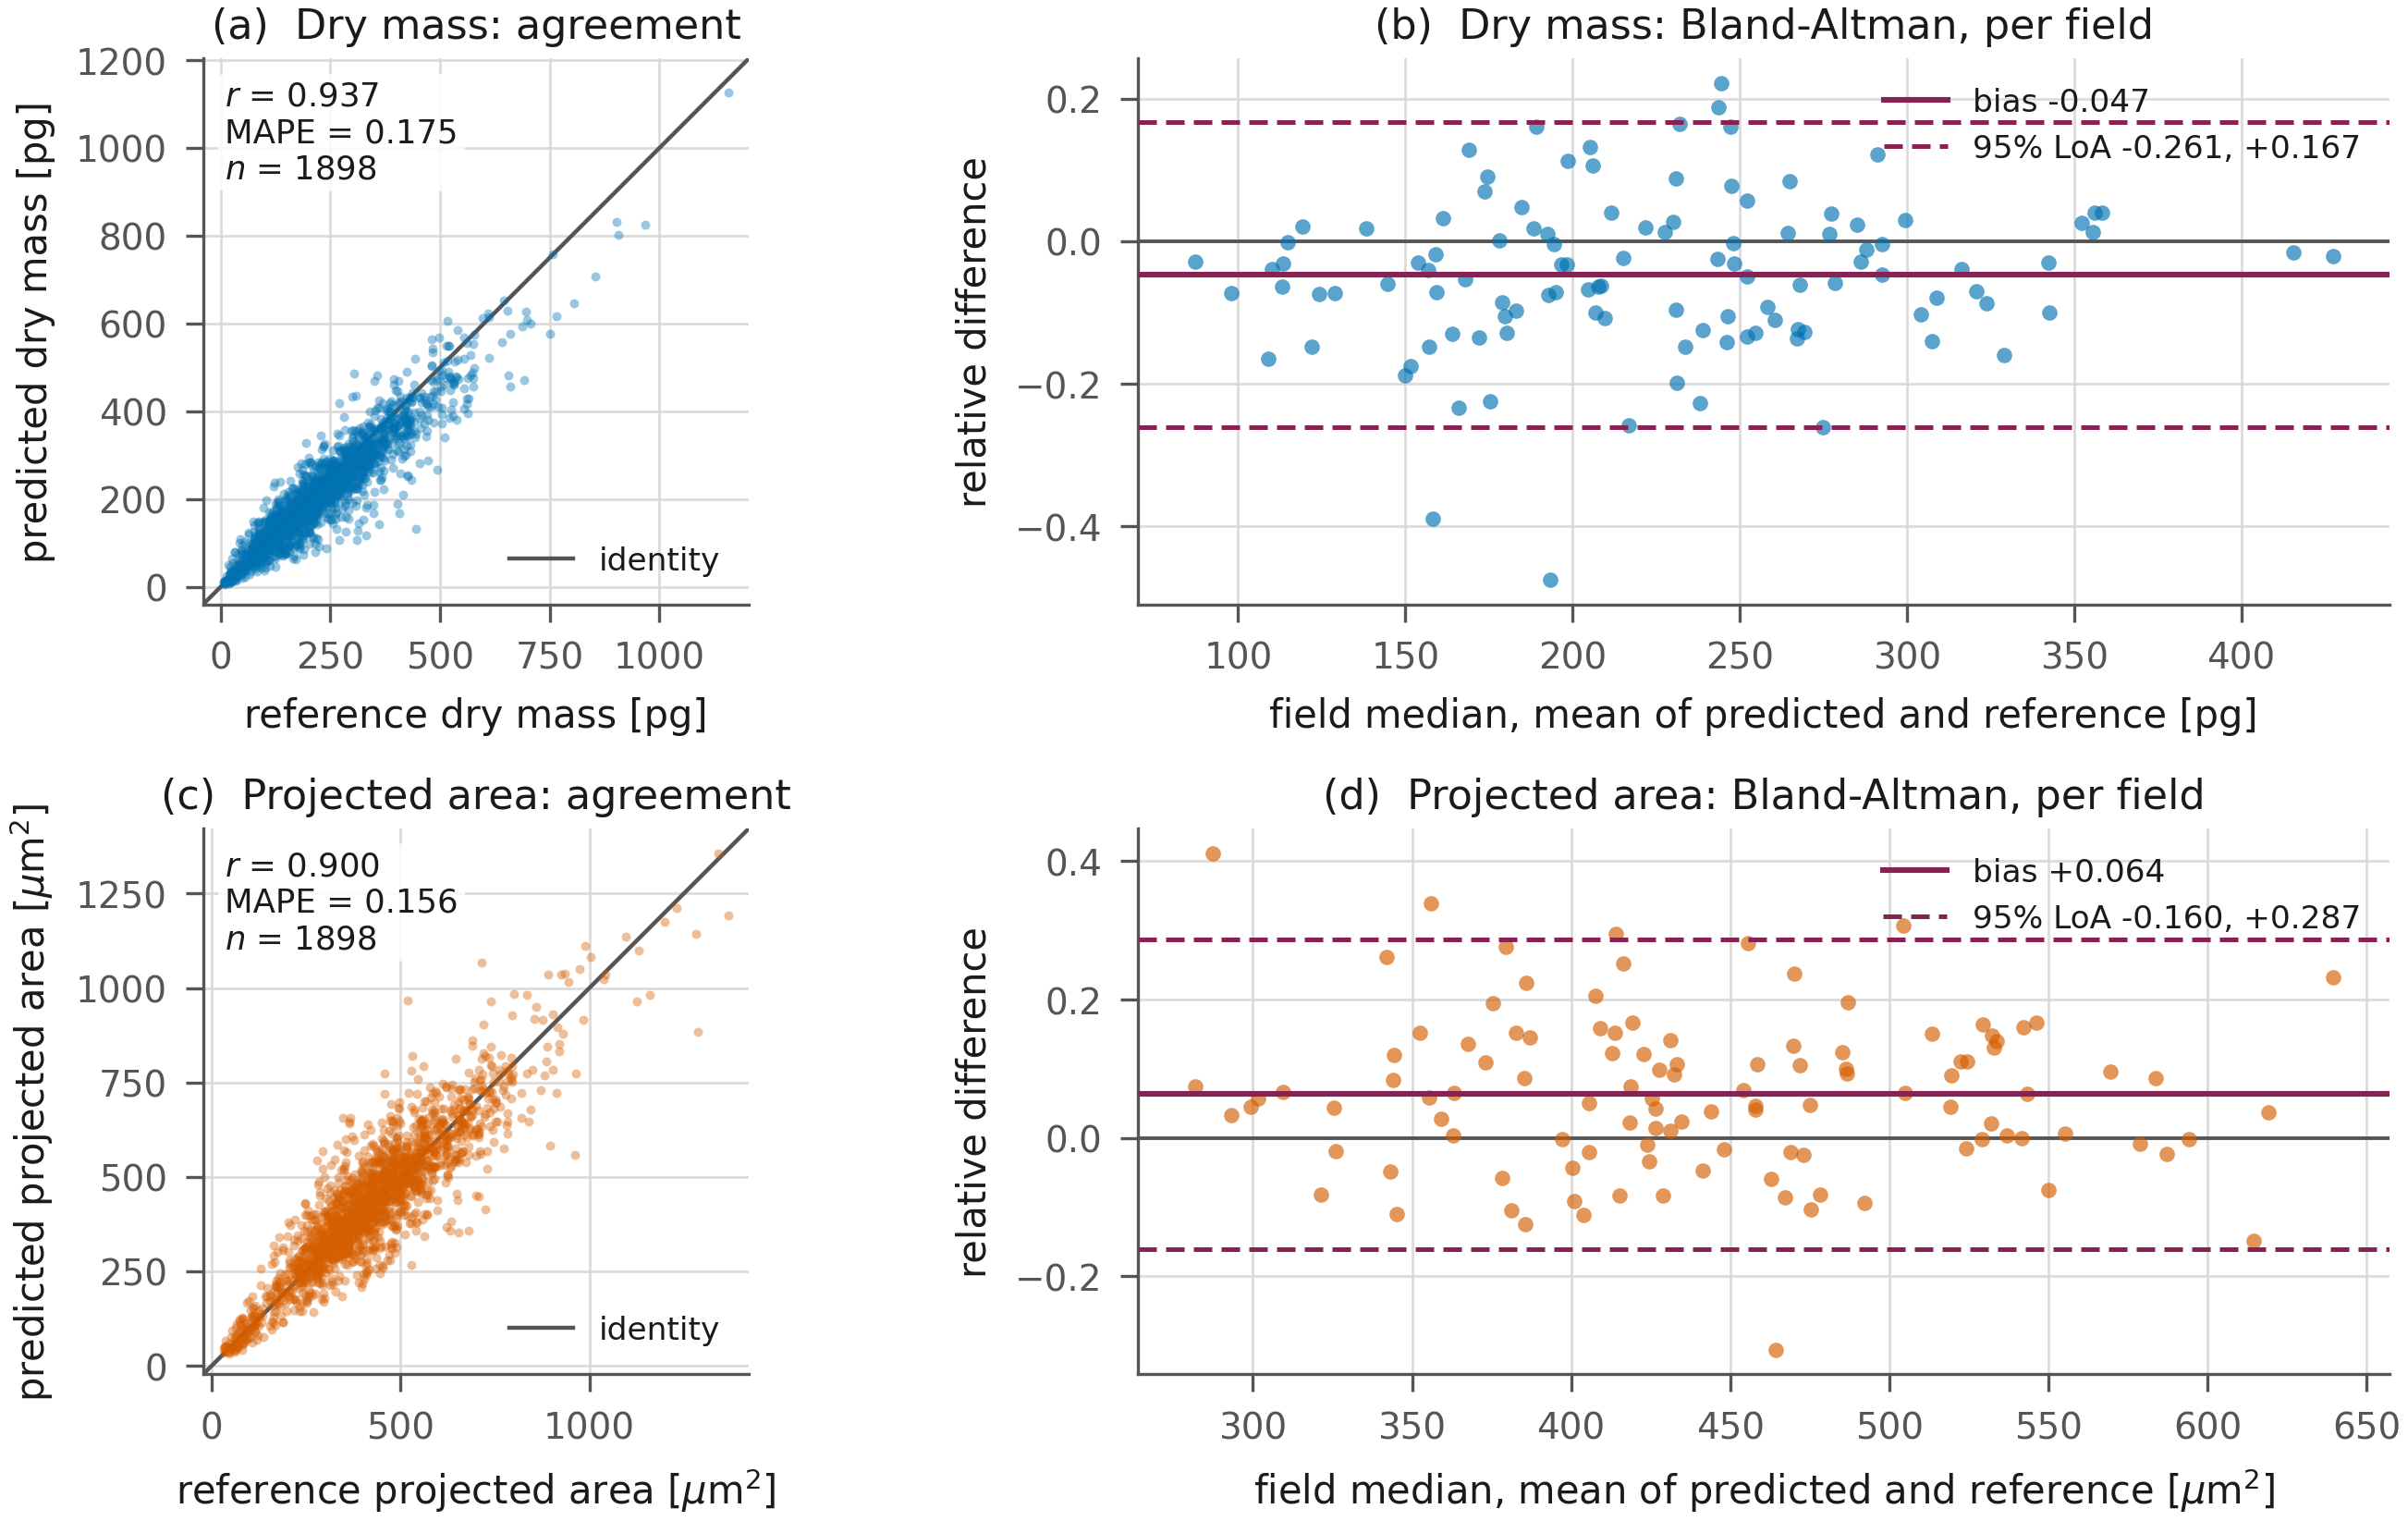
\includegraphics[width=0.78\textwidth]{figure_4.png}
\caption{Per-cell agreement of the seed-42 End-to-End Neural Baseline on the
113 off-axis test fields (1898 matched cells) for dry mass (a, b) and projected
area (c, d): predicted against reference values (a, c) and relative
Bland--Altman plots on per-field medians (b, d). The bias and limits of this run
differ slightly from the three-seed means of Table~\ref{tab:measurement}.}
\label{fig:agreement}
\end{figure}

Table~\ref{tab:decomp} splits the predicted-to-reference dry-mass ratio with
Eq.~\eqref{eq:decomp}. For matched cells of the baseline, the geometric-mean
domain factor is $1.002\pm0.002$ and the phase factor $0.929\pm0.016$, so the
predicted domain encloses almost the same reference phase integral as the
reference domain, and the systematic underestimate of matched cells lies in the
predicted phase level. The phase factor also carries most of the spread
(median $|\log|$ $0.102$ against $0.042$ for the domain factor). The phase
factor is $0.957$ for interior cells and $0.797$ for edge cells. At field level
the domain factor is $0.897$; since the field-level domain includes every
reference cell, this value reflects reference cells that were not detected, in
addition to boundary placement. These statements concern matched cells; with a
recall of $0.593$, a matched-cell domain factor near 1 says nothing about the
cells that were missed.

The tested classical pipeline has a different structure. For matched cells its
domain factor is $0.966$ and its phase factor $1.014$, and at field level
$0.857$ and $1.055$, giving a field-level total of $0.905$ against $0.838$ for
the baseline. Opposing domain and phase deviations thus coincide with the lower
field-total error of the classical pipeline reported in
Sec.~\ref{sec:res-recon}, which indicates a compensatory error structure. The
factors and the field-total MAPE are different summaries, and the factors do
not by themselves account for the MAPE values.

% Table 7: decomposition of the dry-mass ratio into a domain factor and a phase factor.
\begin{table}[!htbp]
\centering
\caption{Decomposition of the predicted-to-reference dry-mass ratio into a
domain factor and a phase factor (Eq.~\eqref{eq:decomp}) on the off-axis test
set (113 fields). GM: geometric mean of the factor (mean $\pm$ SD over three
seeds for the baseline); $|\log|$: median absolute log ratio (spread). Edge:
reference instance with a pixel within 3\,px of the field boundary.}
\label{tab:decomp}
\scriptsize
\begin{tabular*}{\textwidth}{@{\extracolsep{\fill}}lrccccccc@{}}
\toprule
 & & & \multicolumn{3}{c}{GM} & \multicolumn{3}{c}{$|\log|$} \\
\cmidrule(lr){4-6}\cmidrule(lr){7-9}
Level / group & $N$ & Recall & Domain & Phase & Total & Domain & Phase & Total \\
\midrule
\multicolumn{9}{@{}l}{\emph{End-to-End Neural Baseline ($n=3$)}} \\
\quad Matched cells, all & 1889 & 0.593 & $1.002 \pm 0.002$ & $0.929 \pm 0.016$ & $0.931 \pm 0.014$ & 0.042 & 0.102 & 0.132 \\
\quad Matched cells, interior & 1581 & 0.912 & $1.006 \pm 0.002$ & $0.957 \pm 0.017$ & $0.963 \pm 0.015$ & 0.038 & 0.090 & 0.116 \\
\quad Matched cells, edge & 308 & 0.212 & $0.982 \pm 0.004$ & $0.797 \pm 0.014$ & $0.782 \pm 0.014$ & 0.076 & 0.267 & 0.303 \\
\quad Field (foreground) & 113 fields & N/A & $0.897 \pm 0.002$ & $0.933 \pm 0.021$ & $0.838 \pm 0.017$ & 0.105 & 0.073 & 0.179 \\
\midrule
\multicolumn{9}{@{}l}{\emph{Classical pipeline ($n=1$)}} \\
\quad Matched cells, all & 1870 & 0.587 & 0.966 & 1.014 & 0.980 & 0.046 & 0.119 & 0.169 \\
\quad Matched cells, interior & 1543 & 0.890 & 0.977 & 1.028 & 1.004 & 0.041 & 0.106 & 0.152 \\
\quad Matched cells, edge & 327 & 0.225 & 0.919 & 0.952 & 0.875 & 0.095 & 0.212 & 0.308 \\
\quad Field (foreground) & 113 fields & N/A & 0.857 & 1.055 & 0.905 & 0.141 & 0.061 & 0.095 \\
\bottomrule
\end{tabular*}
\tabnote{$N$: matched cells per run (baseline: mean over seeds) or fields; $n$ in the group labels is the number of training runs.
Matched cells are recomputed by the decomposition script and differ from the
stored evaluation by at most three cells per run; the re-scoring gives a per-run
mean of 1889 matched cells, against $1890\pm9$ from the stored evaluation
(Table~\ref{tab:learned-vs-classical}). Field level: the whole
predicted and reference foreground, so undetected and spurious cells enter the
domain factor.}
\end{table}


The matched-cell errors describe the detected cells only. Detection recall is
$0.5931\pm0.0027$, so about 1300 of the 3186 reference cells are not matched,
and the coverage-adjusted dry-mass error is $0.5102$. Stratifying by location
(Table~\ref{tab:edge}) shows that the missed cells are concentrated at the field
boundary. 1452 reference instances (45.6\%) have a pixel within 3\,px of the
boundary. The baseline recalls $0.212$ of these edge instances and $0.912$ of
the interior ones, so about 1140 of the roughly 1300 unmatched reference cells
are edge instances. Its matched-cell dry-mass MAPE is $0.305$ on edge cells and
$0.149$ on interior cells. Edge instances include cells cut by the field
boundary, whose area and mass are physically incomplete, and elongated boundary
regions of the kind visible in Fig.~\ref{fig:qualitative}; they were not
classified individually.

% Table 8: detection and matched-cell error by location of the reference instance.
\begin{table}[!htbp]
\centering
\caption{Detection recall, matched-cell dry-mass MAPE and false positives by
location of the reference instance on the off-axis test set (113 fields; 1452 edge
and 1734 interior reference instances). Neural
configurations: mean $\pm$ SD over three seeds.}
\label{tab:edge}
\footnotesize
\begin{tabular*}{\textwidth}{@{\extracolsep{\fill}}lcccccc@{}}
\toprule
 & \multicolumn{2}{c}{Recall} & \multicolumn{2}{c}{Dry-mass MAPE} & \multicolumn{2}{c}{False positives per run} \\
\cmidrule(lr){2-3}\cmidrule(lr){4-5}\cmidrule(lr){6-7}
Configuration & Edge & Interior & Edge & Interior & All & Within 15\,px \\
\midrule
End-to-End Neural Baseline & $0.212 \pm 0.003$ & $0.912 \pm 0.002$ & $0.305 \pm 0.010$ & $0.149 \pm 0.004$ & $337 \pm 32$ & $136 \pm 16$ \\
+IPP (per-cell) & $0.220 \pm 0.005$ & $0.919 \pm 0.002$ & $0.315 \pm 0.012$ & $0.163 \pm 0.003$ & $456 \pm 40$ & $203 \pm 22$ \\
+IPP (image) & $0.208 \pm 0.000$ & $0.907 \pm 0.003$ & $0.299 \pm 0.009$ & $0.167 \pm 0.003$ & $342 \pm 27$ & $136 \pm 14$ \\
\midrule
Classical pipeline ($n=1$) & 0.225 & 0.890 & 0.322 & 0.199 & 494 & 137 \\
\bottomrule
\end{tabular*}
\tabnote{Edge: reference instance with a pixel within 3\,px of the field
boundary. Within 15\,px: false-positive centroid within 15\,px of the field
boundary. Recall and MAPE are recomputed by the decomposition script (matched
cells within three of the stored evaluation per run).}
\end{table}


Scored against the provisional membrane-derived masks instead of the
phase-derived ones, the baseline's Dice is $0.502$ (against $0.834$), AJI
$0.236$ ($0.671$), boundary F1 $0.064$ ($0.469$) and recall $0.114$ ($0.593$),
means over three seeds with between-seed SD at most $0.002$. The membrane masks
were scored over the whole field, including regions outside the fluorescence
illumination, and they are thresholded perimeter stains. These values do not
replace the phase-derived ones, but they show that agreement with the
phase-derived labels does not carry over to an independent delineation of the
same cells.

\subsection{Measurement-aware training objectives}
\label{sec:res-mawo}

Table~\ref{tab:ablation} lists, for every configuration, the matched-cell
dry-mass MAPE next to the coverage-adjusted and field-total errors and the
intermediate metrics; Table~\ref{tab:seeds} gives the between-seed statistics
of the replicated configurations and every dry-mass difference with its
assessment under the resolution criterion. Figure~\ref{fig:ablation} plots dry-mass MAPE and Dice for
the configurations outside the weight sweep.

% Table 9: ablation over objective terms and decoder capacity (off-axis, 113 test fields).
\begin{table}[!htbp]
\centering
\caption{Ablation over objective terms and decoder capacity on the off-axis
test set (113 fields, 3186 reference cells). $n$: training runs; $n=3$
entries are means over seeds 42, 1337 and 2024, $n=1$ entries are seed-42 runs.}
\label{tab:ablation}
\scriptsize
\begin{tabular*}{\textwidth}{@{\extracolsep{\fill}}lcrrrrrrrr@{}}
\toprule
 & & \multicolumn{3}{c}{Dry-mass MAPE $\downarrow$} & Area & Recall & Precision & Dice & Phase \\
\cmidrule(lr){3-5}
Configuration & $n$ & matched & cov.-adj. & field total & MAPE $\downarrow$ & $\uparrow$ & $\uparrow$ & $\uparrow$ & MAE [rad] $\downarrow$ \\
\midrule
End-to-End Neural Baseline & 3 & 0.1742 & 0.5102 & 0.1631 & 0.1568 & 0.5931 & 0.8488 & 0.8337 & 0.1568 \\
\midrule
+IPP (per-cell) & 3 & 0.1883 & 0.5125 & 0.1676 & 0.1679 & 0.6006 & 0.8077 & 0.8294 & 0.1656 \\
+IPP (image) & 3 & 0.1887 & 0.5222 & 0.1722 & 0.1597 & 0.5889 & 0.8460 & 0.8294 & 0.1644 \\
+Area & 1 & 0.1850 & 0.5075 & 0.1696 & 0.1779 & 0.6042 & 0.7958 & 0.8294 & 0.1646 \\
+BGA & 1 & 0.1921 & 0.5182 & 0.1651 & 0.1652 & 0.5964 & 0.8183 & 0.8309 & 0.1654 \\
\midrule
+IPP (per-cell), $w=0.1$ & 1 & 0.1754 & 0.5158 & 0.1830 & 0.1504 & 0.5873 & 0.8428 & 0.8331 & 0.1567 \\
+IPP (per-cell), $w=0.3$ & 1 & 0.1881 & 0.5196 & 0.1953 & 0.1564 & 0.5917 & 0.8389 & 0.8328 & 0.1620 \\
+IPP (per-cell), $w=1.0$ & 3 & 0.1883 & 0.5125 & 0.1676 & 0.1679 & 0.6006 & 0.8077 & 0.8294 & 0.1656 \\
+IPP (per-cell), $w=3.0$ & 1 & 0.1963 & 0.5197 & 0.1316 & 0.1729 & 0.5976 & 0.7855 & 0.8164 & 0.1813 \\
\midrule
+Amplitude & 1 & 0.1857 & 0.5157 & 0.1528 & 0.1591 & 0.5948 & 0.8282 & 0.8297 & 0.1633 \\
+Fwd (fixed $z$) & 1 & 0.1855 & 0.5081 & 0.1573 & 0.1685 & 0.6039 & 0.8297 & 0.8318 & 0.1647 \\
+Fwd (free $z$) & 1 & 0.1920 & 0.5212 & 0.1599 & 0.1583 & 0.5926 & 0.8248 & 0.8290 & 0.1636 \\
\midrule
Compact Baseline & 1 & 0.1740 & 0.5123 & 0.1738 & 0.1508 & 0.5904 & 0.8496 & 0.8345 & 0.1562 \\
Compact +IPP & 1 & 0.1887 & 0.5088 & 0.1539 & 0.1656 & 0.6055 & 0.8174 & 0.8306 & 0.1652 \\
\bottomrule
\end{tabular*}
\tabnote{Differences from a single run ($n=1$) are not resolvable under the
between-seed criterion (Sec.~\ref{sec:stats}). Field totals sum all predicted
and all reference cells and are dominated by the coverage deficit: the
field-total dry-mass bias is negative in every configuration (Table~\ref{tab:seeds}a
for the replicated ones). The $w=1.0$ row repeats +IPP (per-cell); a separate
seed-42 training of the identical configuration gave a matched-cell MAPE of
0.1872 (seed-42 run of +IPP (per-cell): 0.1875).}
\end{table}


Both measurement-aware integrated-phase terms increased matched-cell dry-mass
MAPE (+IPP (per-cell) $\Delta=+0.0141$, $2\times$SD $0.0097$; +IPP (image)
$\Delta=+0.0145$, $2\times$SD $0.0066$; both resolved under the predefined
between-seed criterion). The two forms differ by $+0.0004$, inside their
$2\times$SD of $0.0076$. Their effect on field-total dry-mass MAPE was not
resolved ($+0.0045$, $2\times$SD $0.0232$; $+0.0091$, $2\times$SD $0.0250$).
Several intermediate metrics also moved in the unfavourable direction by
resolved amounts. Under +IPP (per-cell) these were area MAPE, phase MAE over the
field and inside cells, phase $r$, SSIM, AJI, boundary F1 and precision
($0.8488\rightarrow0.8077$), with $119$ more false-positive cells per run;
under +IPP (image) they were phase MAE over the field and inside cells, phase
$r$, SSIM, Dice, AJI and boundary F1. +IPP (per-cell) also raised recall by
$0.0075$ (resolved), and at field level its domain factor rose from $0.897$ to
$0.909$ ($+0.0118$, $2\times$SD $0.0081$, resolved), together with the
additional false positives, $67$ of which per run have centroids within 15\,px
of the field boundary (Table~\ref{tab:edge}).

\begin{figure}[!htbp]
\centering
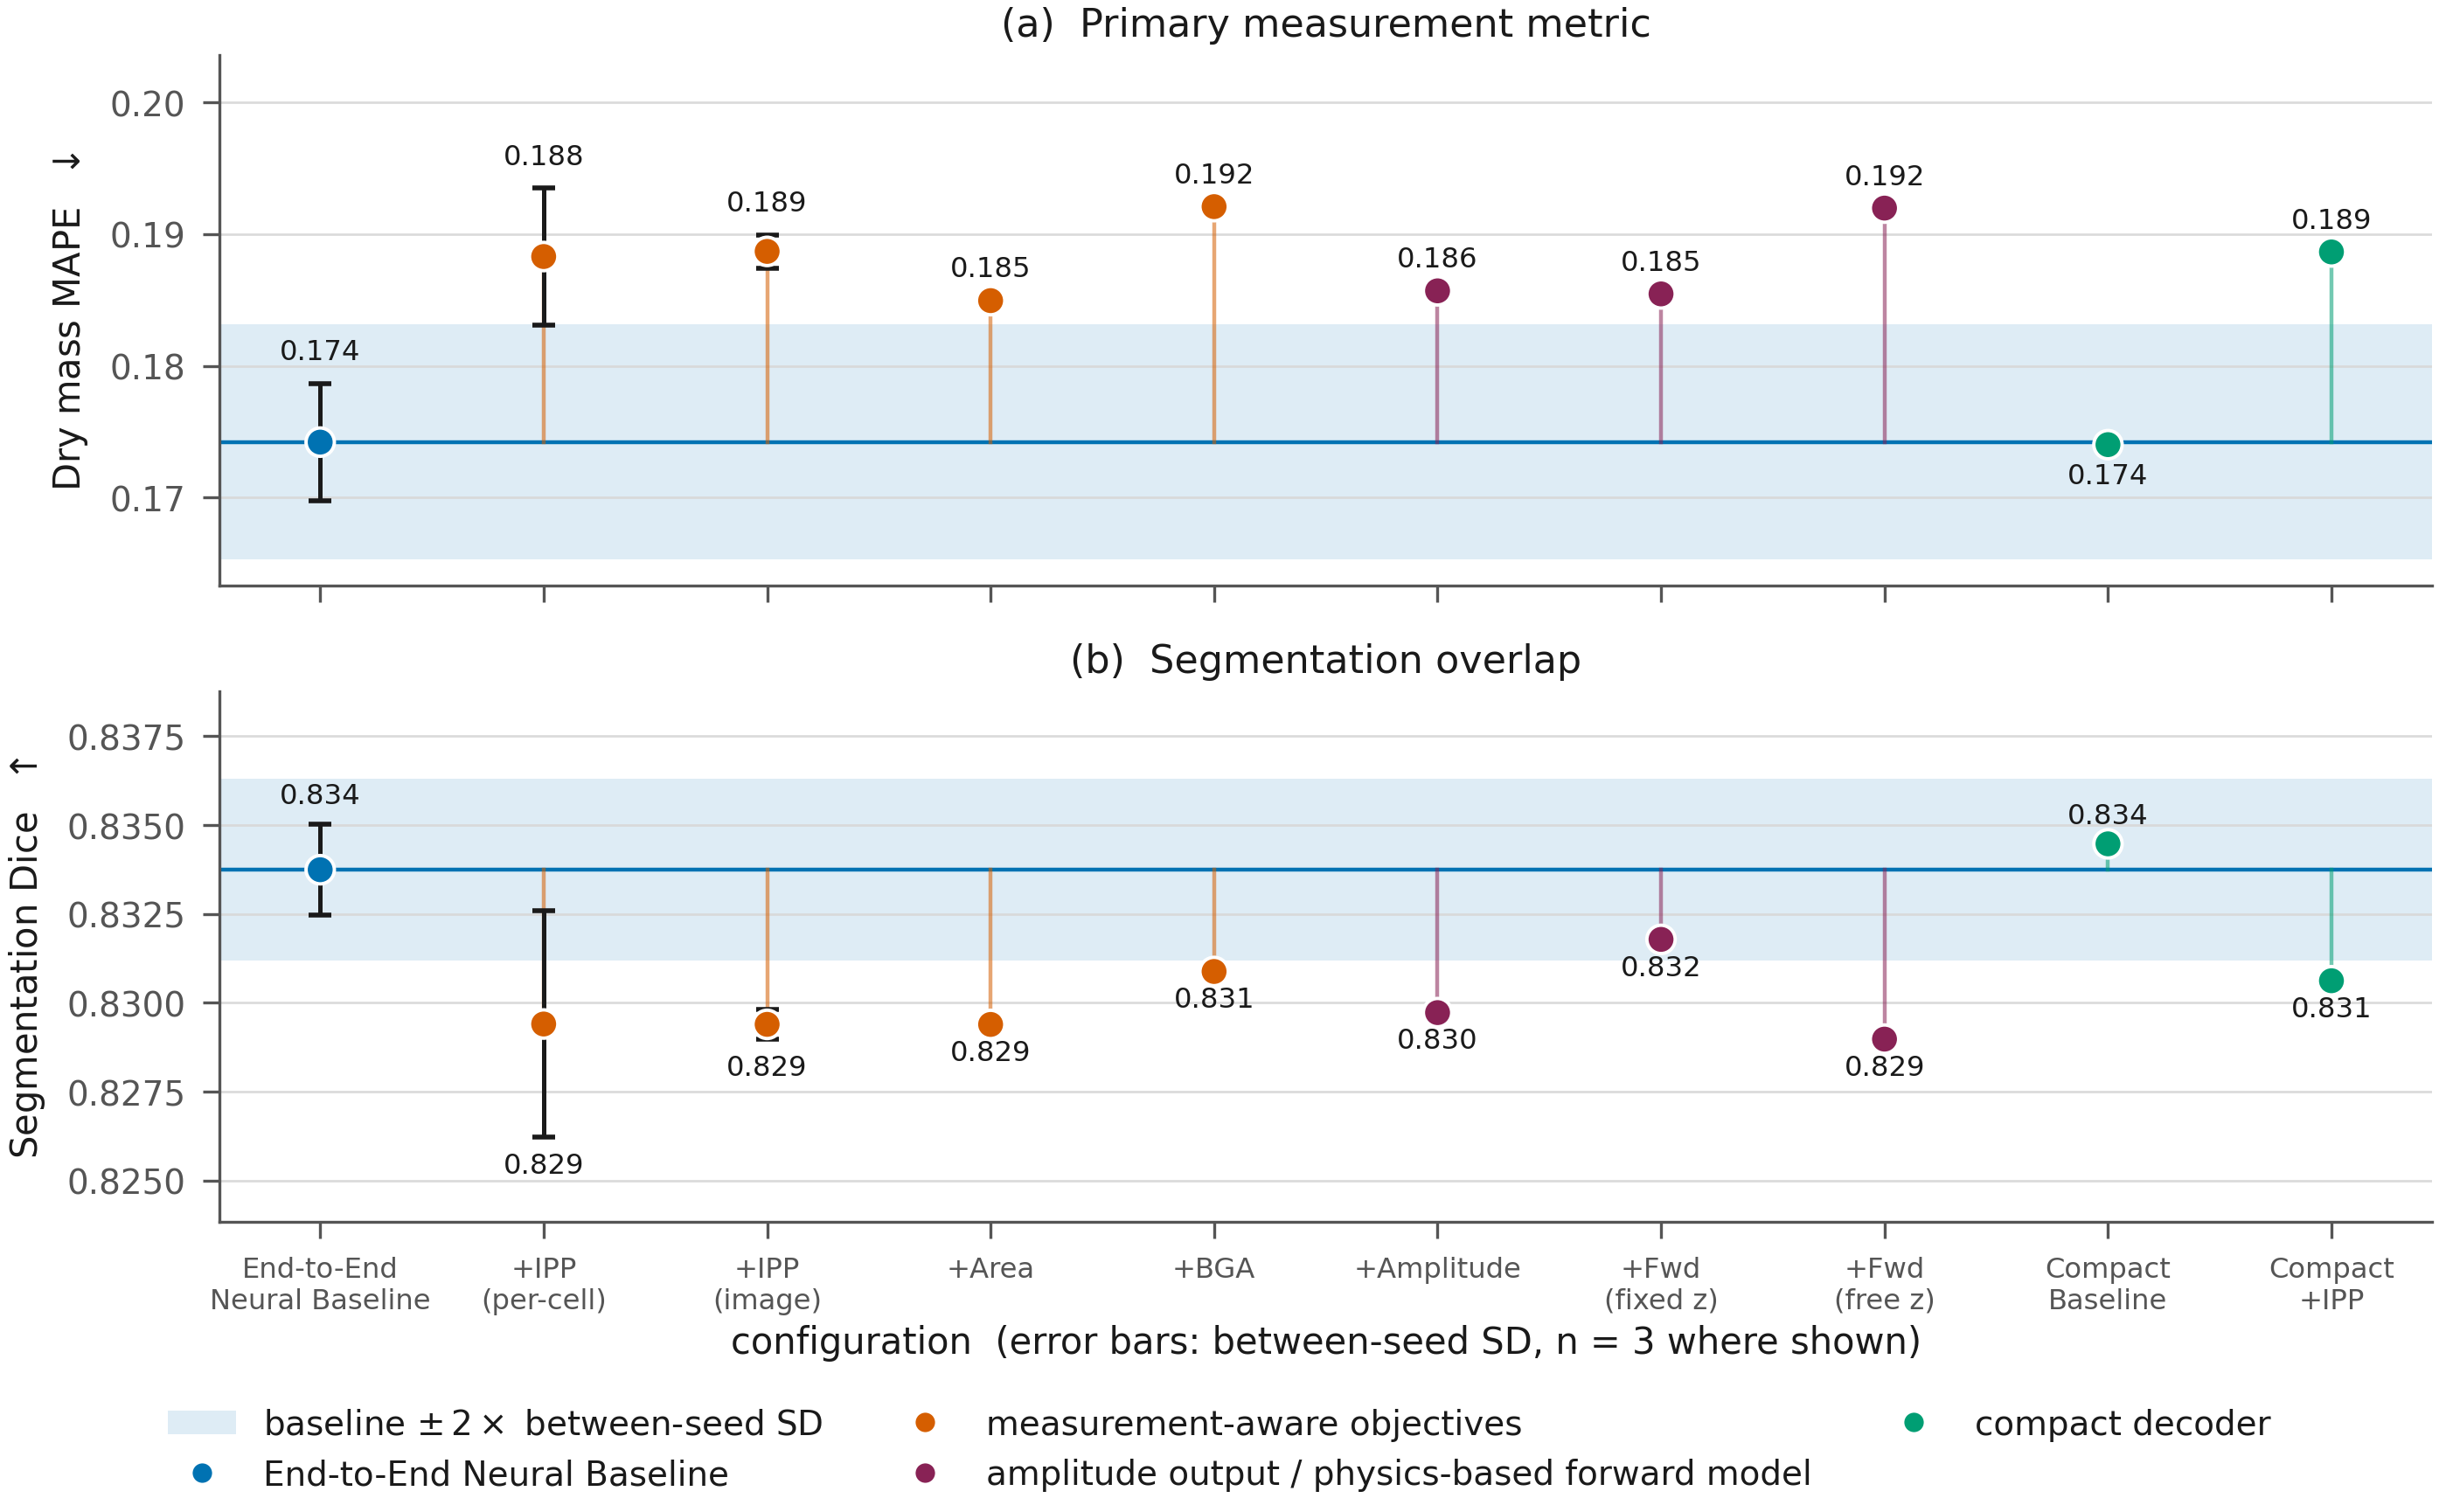
\includegraphics[width=0.8\textwidth]{figure_5.png}
\caption{(a) Matched-cell dry-mass MAPE and (b) Dice of the off-axis
configurations on the 113 test fields. Error bars: between-seed SD for the
three configurations with three runs; other points are single runs. Shaded
band: baseline mean $\pm2\times$ its between-seed SD. Vertical axes do not start
at zero.}
\label{fig:ablation}
\end{figure}

% Table 10: between-seed variability and resolution of differences.
\begin{table}[!htbp]
\centering
\caption{Replicated configurations on the off-axis test set (113 fields). (a)
Mean $\pm$ SD over seeds 42, 1337 and 2024. (b) Differences in matched-cell and
field-total dry-mass MAPE, configuration minus comparator, with $2\times$ the pooled between-seed SD
and the assessment.}
\label{tab:seeds}
\footnotesize
\textbf{(a) Mean $\pm$ SD over three seeds}\\[2pt]
\begin{tabular*}{\textwidth}{@{\extracolsep{\fill}}lccc@{}}
\toprule
Metric & Baseline & +IPP (per-cell) & +IPP (image) \\
\midrule
Dry-mass MAPE & $0.1742 \pm 0.0045$ & $0.1883 \pm 0.0052$ & $0.1887 \pm 0.0013$ \\
Field-total dry-mass MAPE & $0.1631 \pm 0.0141$ & $0.1676 \pm 0.0084$ & $0.1722 \pm 0.0107$ \\
Field-total dry-mass bias & $-0.1560 \pm 0.0174$ & $-0.1496 \pm 0.0181$ & $-0.1667 \pm 0.0078$ \\
Area MAPE & $0.1568 \pm 0.0027$ & $0.1679 \pm 0.0059$ & $0.1597 \pm 0.0014$ \\
Phase MAE [rad] & $0.1568 \pm 0.0023$ & $0.1656 \pm 0.0032$ & $0.1644 \pm 0.0015$ \\
Phase MAE inside cells [rad] & $0.2689 \pm 0.0056$ & $0.2876 \pm 0.0064$ & $0.2946 \pm 0.0039$ \\
Phase $r$ & $0.8741 \pm 0.0023$ & $0.8636 \pm 0.0019$ & $0.8655 \pm 0.0005$ \\
Dice & $0.8337 \pm 0.0013$ & $0.8294 \pm 0.0032$ & $0.8294 \pm 0.0004$ \\
AJI & $0.6710 \pm 0.0025$ & $0.6616 \pm 0.0059$ & $0.6632 \pm 0.0009$ \\
Boundary F1 & $0.4687 \pm 0.0053$ & $0.4518 \pm 0.0093$ & $0.4477 \pm 0.0028$ \\
Detection recall & $0.5931 \pm 0.0027$ & $0.6006 \pm 0.0034$ & $0.5889 \pm 0.0013$ \\
Detection precision & $0.8488 \pm 0.0124$ & $0.8077 \pm 0.0138$ & $0.8460 \pm 0.0100$ \\
False positives per run & $337 \pm 32$ & $456 \pm 40$ & $342 \pm 27$ \\
\bottomrule
\end{tabular*}

\vspace{8pt}
\textbf{(b) Differences}\\[2pt]
\begin{tabular*}{\textwidth}{@{\extracolsep{\fill}}lrrl@{}}
\toprule
Comparison & $\Delta$ & $2\times$ pooled SD & Assessment \\
\midrule
\multicolumn{4}{@{}l}{\emph{Matched-cell dry-mass MAPE; both configurations with three training runs}} \\
+IPP (per-cell) vs Baseline & $\mathbf{+0.0141}$ & 0.0097 & Exceeds $2\times$ pooled SD \\
+IPP (image) vs Baseline & $\mathbf{+0.0145}$ & 0.0066 & Exceeds $2\times$ pooled SD \\
+IPP (image) vs +IPP (per-cell) & $+0.0004$ & 0.0076 & Within $2\times$ pooled SD \\
\midrule
\multicolumn{4}{@{}l}{\emph{At least one configuration with a single training run}} \\
+Area vs +IPP (per-cell) & $-0.0033$ & N/A & Not estimable from the available runs \\
+BGA vs +IPP (per-cell) & $+0.0038$ & N/A & Not estimable from the available runs \\
$w=0.1$ vs Baseline & $+0.0012$ & N/A & Not estimable from the available runs \\
$w=0.3$ vs Baseline & $+0.0138$ & N/A & Not estimable from the available runs \\
$w=3.0$ vs Baseline & $+0.0221$ & N/A & Not estimable from the available runs \\
+Amplitude vs +IPP (per-cell) & $-0.0026$ & N/A & Not estimable from the available runs \\
+Fwd (fixed $z$) vs +Amplitude & $-0.0002$ & N/A & Not estimable from the available runs \\
+Fwd (free $z$) vs +Fwd (fixed $z$) & $+0.0065$ & N/A & Not estimable from the available runs \\
Compact Baseline vs Baseline & $-0.0002$ & N/A & Not estimable from the available runs \\
Compact +IPP vs +IPP (per-cell) & $+0.0003$ & N/A & Not estimable from the available runs \\
\midrule
\multicolumn{4}{@{}l}{\emph{Field-total dry-mass MAPE; both configurations with three training runs}} \\
+IPP (per-cell) vs Baseline & $+0.0045$ & 0.0232 & Within $2\times$ pooled SD \\
+IPP (image) vs Baseline & $+0.0091$ & 0.0250 & Within $2\times$ pooled SD \\
+IPP (image) vs +IPP (per-cell) & $+0.0046$ & 0.0193 & Within $2\times$ pooled SD \\
\midrule
\multicolumn{4}{@{}l}{\emph{At least one configuration with a single training run}} \\
+Area vs +IPP (per-cell) & $+0.0020$ & N/A & Not estimable from the available runs \\
+BGA vs +IPP (per-cell) & $-0.0025$ & N/A & Not estimable from the available runs \\
$w=0.1$ vs Baseline & $+0.0199$ & N/A & Not estimable from the available runs \\
$w=0.3$ vs Baseline & $+0.0322$ & N/A & Not estimable from the available runs \\
$w=3.0$ vs Baseline & $-0.0315$ & N/A & Not estimable from the available runs \\
+Amplitude vs +IPP (per-cell) & $-0.0148$ & N/A & Not estimable from the available runs \\
+Fwd (fixed $z$) vs +Amplitude & $+0.0046$ & N/A & Not estimable from the available runs \\
+Fwd (free $z$) vs +Fwd (fixed $z$) & $+0.0025$ & N/A & Not estimable from the available runs \\
Compact Baseline vs Baseline & $+0.0107$ & N/A & Not estimable from the available runs \\
Compact +IPP vs +IPP (per-cell) & $-0.0137$ & N/A & Not estimable from the available runs \\
\bottomrule
\end{tabular*}
\tabnote{$\Delta$: configuration minus comparator; positive is worse. Bold: $|\Delta| > 2\sqrt{(s_1^2+s_2^2)/2}$ with $s$ the
between-seed SD of each configuration, both configurations having at least three training runs. Not estimable: fewer than three
training runs on one side, so no between-seed SD exists; no other variance is substituted. Differences are computed from unrounded means.}
\end{table}


The decomposition did not localise the increase consistently. No change in the
geometric-mean domain or phase factor was resolved for all matched cells under
either term, and the only resolved change in spread over all matched cells was
a $+0.0025$ increase of the domain $|\log|$ spread under +IPP (image). The
changes that were resolved are mostly for +IPP (image) and point in different
directions for interior and edge cells: its interior phase spread rose by
$0.0177$, while its edge phase spread fell by $0.0352$ and its edge phase factor
rose by $0.0374$. Under +IPP (per-cell) the resolved changes are a higher edge
domain factor ($+0.0154$) and edge total ($+0.0341$). By location, the
matched-cell MAPE increase is resolved among interior cells for both terms
($+0.0139$ and $+0.0183$) and not among edge cells (Table~\ref{tab:edge}). The
matched-cell domain factor did not change, so the route allowed by the
formulation of Sec.~\ref{sec:obj-mawo}, a foreground receding inside the
reference domain with a raised phase, was not observed.

+Area and +BGA, each added to +IPP (per-cell), give dry-mass MAPE $0.1850$ and
$0.1921$. Across the weight sweep (Fig.~\ref{fig:sweep}) the MAPE is $0.1754$,
$0.1881$, $0.1883$ and $0.1963$ for $w=0.1$, $0.3$, $1.0$ and $3.0$, and at
$w=3.0$ Dice ($0.8164$), precision ($0.7855$) and phase MAE ($0.1813$\,rad) are
the worst of the sweep. +Amplitude, the two +Fwd configurations, the Compact
Baseline and Compact +IPP give $0.1857$, $0.1855$, $0.1920$, $0.1740$ and
$0.1887$. All of these are single runs, so none of their differences is
resolvable. A separate seed-42 training of the configuration identical to
+IPP (per-cell) gave $0.1872$, against $0.1875$ for the seed-42 run of
+IPP (per-cell).

\begin{figure}[!htbp]
\centering
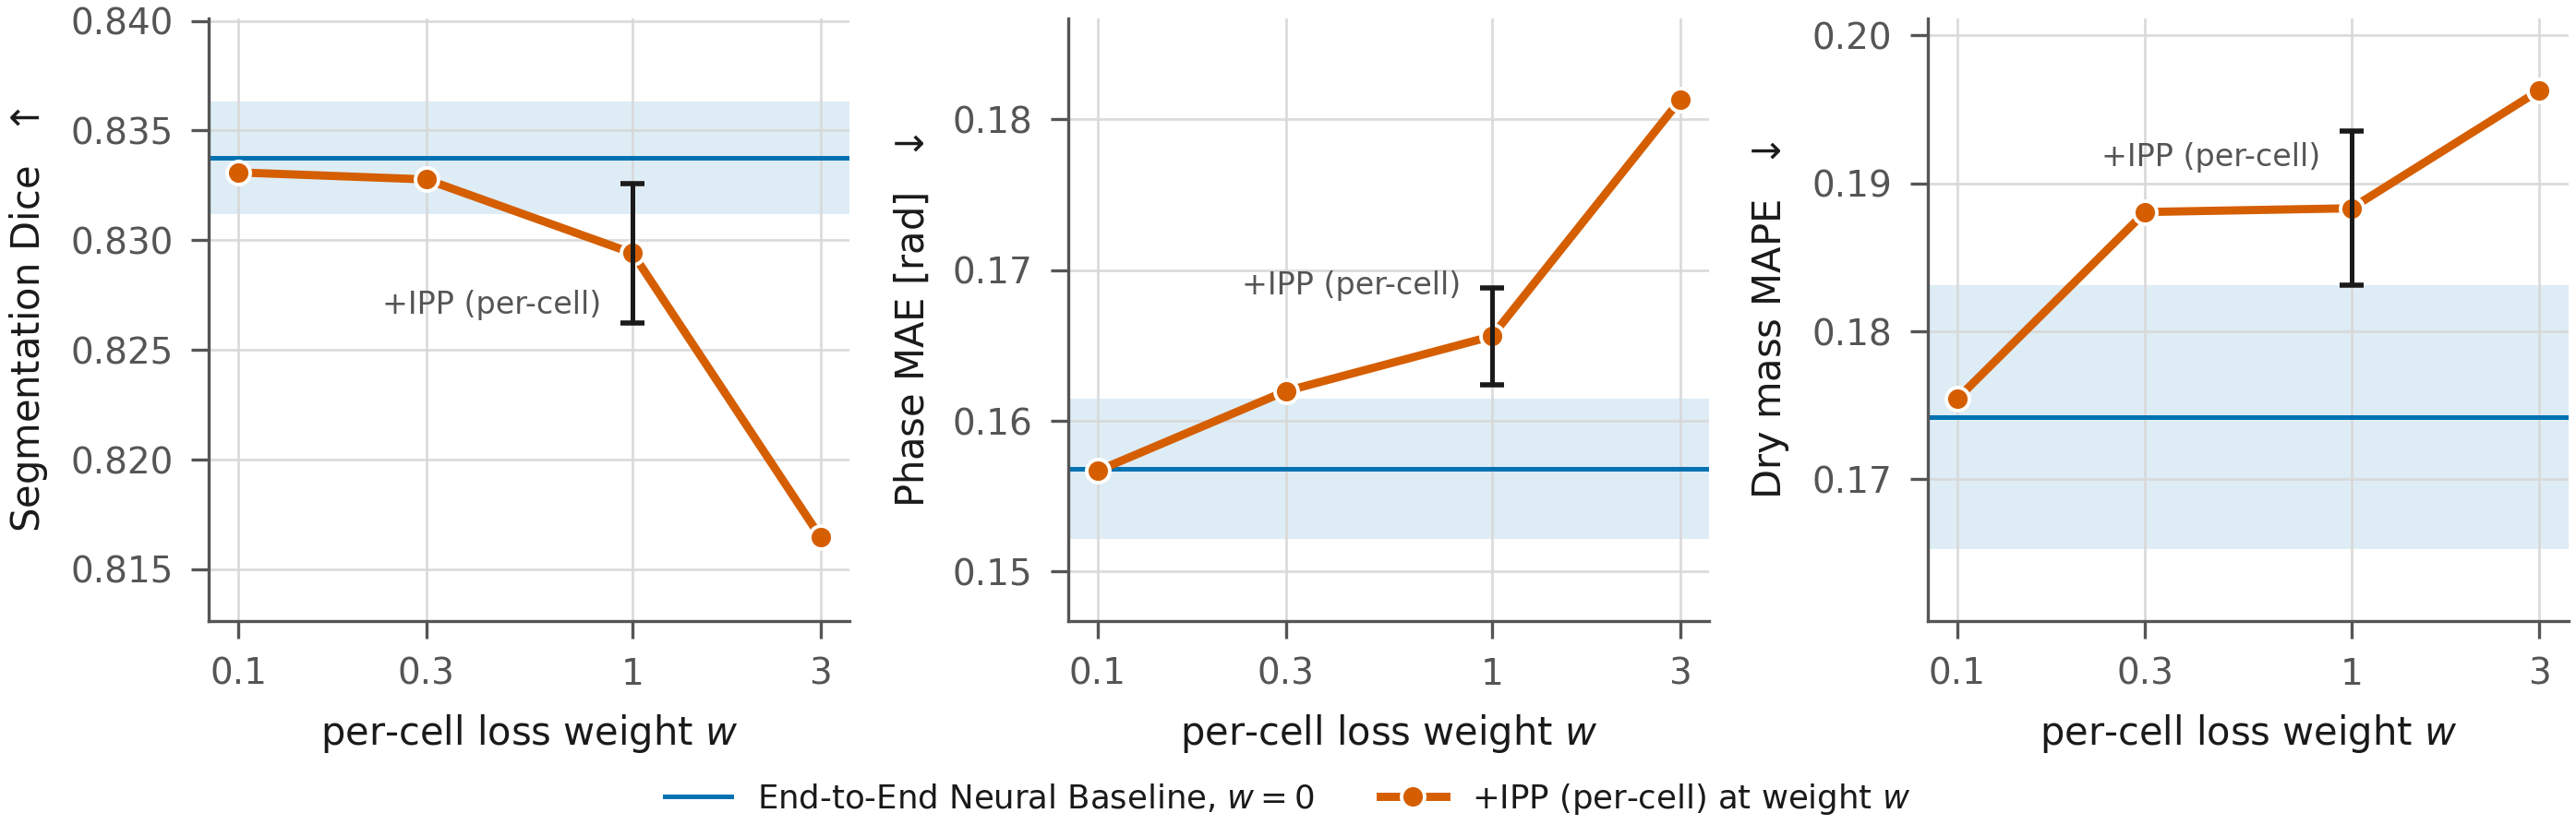
\includegraphics[width=0.92\textwidth]{figure_6.png}
\caption{Segmentation Dice (left), phase MAE (centre) and matched-cell dry-mass
MAPE (right) on the 113 off-axis test fields as functions of the
$\Lippc$ weight. The $w=1.0$ point is +IPP (per-cell), mean $\pm$ SD over three
seeds; the others are single runs. Line and band: baseline mean and
$\pm2\times$ its between-seed SD.}
\label{fig:sweep}
\end{figure}

\subsection{Amplitude prediction}
\label{sec:res-amp}

The amplitude head produces a non-constant transmittance map (predicted SD
$0.1207$ for +Amplitude) that agrees with the reconstruction-derived amplitude
reference at an MAE of $0.0651$ and a Pearson $r$ of $0.9047$, against an MAE of
$0.1469$ for the unit-amplitude assumption $A=1$, a ratio of $0.443$
(Table~\ref{tab:amplitude}a). The two +Fwd configurations give $0.0665$ and
$0.0651$ (ratios $0.453$ and $0.444$). These configurations were each trained
once, and this is agreement with the output of one classical reconstruction,
not with a measured transmittance. Dry mass depends on the amplitude only
indirectly, through the shared encoder and phase decoder and through $\Lfwd$.
Adding the amplitude output to +IPP (per-cell) changed the dry-mass MAPE by
$-0.0026$, a single-run difference that is not resolvable.

% Table 11: amplitude output, forward-model residual and phase-scale probes.
\begin{table}[!htbp]
\centering
\caption{(a) Amplitude output against the reconstruction-derived amplitude
reference (113 off-axis test fields; one run each). (b) Forward-model residual
on the 113 off-axis test fields (Baseline and +IPP (per-cell): mean $\pm$ SD
over three seeds; others one run). (c) Change in the residual when the
reference phase is scaled by 0.9 or 0.5 (margin: scaled minus reference;
positive means the reference phase has the lower residual).}
\label{tab:amplitude}
\footnotesize
\textbf{(a) Amplitude output}\\[2pt]
\begin{tabular*}{\textwidth}{@{\extracolsep{\fill}}lrrr@{}}
\toprule
Quantity & +Amplitude & +Fwd (fixed $z$) & +Fwd (free $z$) \\
\midrule
MAE vs the reference & 0.0651 & 0.0665 & 0.0651 \\
\quad the same MAE for $A=1$ & 0.1469 & 0.1469 & 0.1469 \\
\quad ratio ($<1$: closer than $A=1$) & 0.4429 & 0.4526 & 0.4436 \\
MAE inside cells & 0.0906 & 0.0922 & 0.0898 \\
Bias & $+0.0339$ & $+0.0378$ & $+0.0323$ \\
Pearson $r$ & 0.9047 & 0.9064 & 0.9045 \\
Predicted amplitude, mean & 1.0324 & 1.0363 & 1.0308 \\
Predicted amplitude, SD & 0.1207 & 0.1223 & 0.1200 \\
Reference amplitude, mean & 0.9985 & 0.9985 & 0.9985 \\
\bottomrule
\end{tabular*}

\vspace{8pt}
\textbf{(b) Forward-model residual}\\[2pt]
\begin{tabular*}{\textwidth}{@{\extracolsep{\fill}}lccccc@{}}
\toprule
Quantity & Baseline & +IPP (per-cell) & +Amplitude & +Fwd (fixed $z$) & +Fwd (free $z$) \\
\midrule
Residual, prediction & $0.8948 \pm 0.0002$ & $0.8968 \pm 0.0005$ & 0.8699 & 0.8702 & 0.8699 \\
Residual, reference phase & $0.8914 \pm 0.0000$ & $0.8914 \pm 0.0000$ & 0.8647 & 0.8643 & 0.8640 \\
Ratio (1.0 = reference phase) & $1.0039 \pm 0.0002$ & $1.0061 \pm 0.0005$ & 1.0061 & 1.0068 & 1.0068 \\
In-cell phase MAE [rad] & $0.2689 \pm 0.0056$ & $0.2876 \pm 0.0064$ & 0.2862 & 0.2893 & 0.2886 \\
\bottomrule
\end{tabular*}

\vspace{8pt}
\textbf{(c) Phase-scale probes}\\[2pt]
\begin{tabular*}{\textwidth}{@{\extracolsep{\fill}}l>{\raggedleft\arraybackslash}p{1.5cm}rp{2.4cm}rp{2.4cm}@{}}
\toprule
 & & \multicolumn{2}{c}{$0.9\times$ phase} & \multicolumn{2}{c}{$0.5\times$ phase} \\
\cmidrule(lr){3-4}\cmidrule(lr){5-6}
Geometry and fields & Residual & Margin & Fields favouring reference phase & Margin & Fields favouring reference phase \\
\midrule
Off-axis, 32 validation fields & 0.9147 & $+0.00035$ & 18/32 & $+0.0080$ & 20/32 \\
In-line, 32 validation fields & 0.6993 & $+0.00432$ & 30/32 & $+0.0622$ & 32/32 \\
Off-axis, 113 test fields, global surface & 0.8914 & $+0.00027$ & 60/113 & $+0.0070$ & 71/113 \\
Off-axis, 112 test fields, per-field surfaces$^{\ast}$ & 0.3906 & $+0.00110$ & 93/112 & $+0.0359$ & 110/112 \\
\bottomrule
\end{tabular*}
\tabnote{Fields favouring reference phase: number of fields on which the scaled phase gives the higher residual than the reference
phase (a count of fields, not a separate test). Margin: scaled minus reference residual, averaged over the fields. Configured tolerance for
a usable margin: 0.01. Residual levels in (b) for configurations with an amplitude output use the predicted amplitude in place of
$A=1$ and are not comparable with the others; only the ratio is. $^{\ast}$Per-field aberration surfaces are fitted against each
field's reference phase and are not available at inference. One test field (T24\_Staurosporine\_100nM\_10) has
no per-field surface: its fit was rejected because the fitted surface exceeded the 45\,rad peak-to-valley limit (405\,rad).
With the global surface on the same 112 fields the residual is 0.8926, the margins are
$+0.00025$ and $+0.0067$ and the counts 59/112 and 70/112.}
\end{table}


\subsection{Forward-model consistency}
\label{sec:res-fwd}

With the reference phase and the global aberration surface, the off-axis
residual of Eq.~\eqref{eq:lfwd} is $0.8914$ on the 113 test fields
(Table~\ref{tab:amplitude}b): the forward model leaves most of the recorded
hologram's variance unexplained even for the reference phase. The network's
predictions come within 1\% of that value. The ratio to the reference-phase
residual lies between $1.0038$ and $1.0094$ for all 13 trained off-axis
configurations (Fig.~\ref{fig:forward}a), $1.0039\pm0.0002$ for the baseline,
which never optimised the term. +Fwd (fixed $z$) and +Fwd (free $z$) have
ratios of $1.0068$ and $1.0068$, against $1.0061$ for +Amplitude, and in-cell
phase MAE of $0.2893$ and $0.2886$\,rad against $0.2689$ for the baseline;
these are single runs. For the In-Line Neural Configuration (one run, 107
fields) the residual of the prediction is $0.7573$ against $0.7654$ for the
reference phase.

Direct probes of the operator give the same picture
(Table~\ref{tab:amplitude}c). On 32 validation fields at the recording distance,
the reference phase leaves a residual of $0.915$ off-axis and $0.699$ in-line.
Scaling the reference phase by $0.9$ raises the residual by $0.00035$ off-axis
(higher on 18 of the 32 fields) and by $0.0043$ in-line (30 of 32); scaling it
by $0.5$ raises it by $0.0080$ off-axis (20 of 32) and by $0.0622$ in-line (32 of
32). Only the
in-line $0.5\times$ margin exceeds the configured tolerance of $0.01$. On the 113
off-axis test fields, the $0.9\times$ and $0.5\times$ rescalings change the
residual by $+0.00027$ and $+0.0070$ with the global surface (higher than the
reference-phase residual on 60 and 71 of the 113 fields); with per-field
surfaces, which are fitted against each field's reference phase and are not
available at inference and exist for 112 of the 113 fields
(Table~\ref{tab:amplitude}c), the residual is $0.391$ and the changes are
$+0.0011$ and $+0.0359$ (93 and 110 of the 112 fields). The per-field best-fitting phase scale has a median of $0.975$
(IQR $0.575$) off-axis and $1.00$ (IQR $0.05$) in-line. Under the implemented
operator the residual therefore did not resolve the phase scale near the
reference in either geometry.

\begin{figure}[!htbp]
\centering
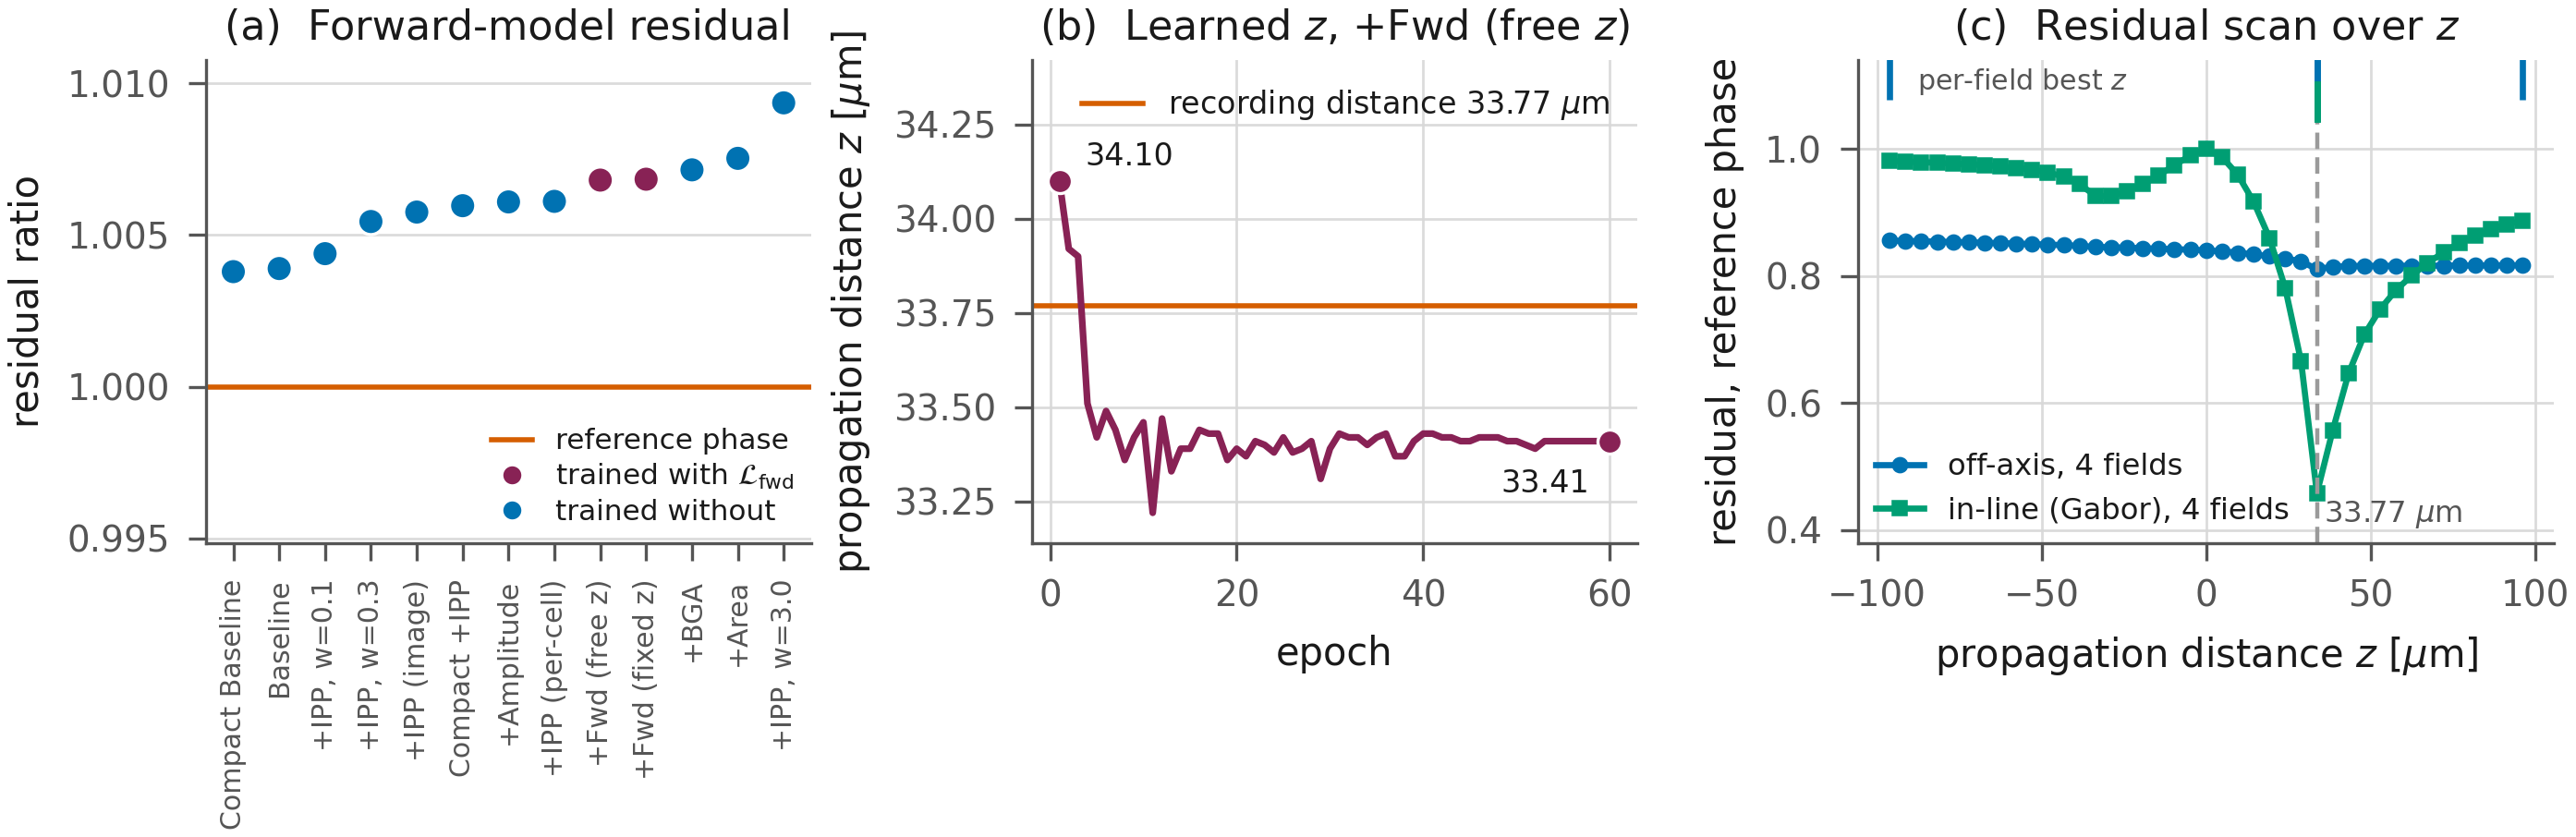
\includegraphics[width=\textwidth]{figure_7.png}
\caption{Forward-model consistency. (a) Residual of each trained off-axis
configuration on the 113 test fields divided by the residual obtained with the
reference phase (three-seed means for the baseline and the two +IPP
configurations, single runs otherwise). (b) Propagation distance of +Fwd
(free $z$) per epoch, initialised at the recording distance. (c) Residual
computed from the reference phase as a function of $z$ on four validation
fields per geometry ($4.81\,\mu$m grid); ticks at the top mark each field's
best distance, and the dashed line the recording distance.}
\label{fig:forward}
\end{figure}

With $z$ trainable and initialised at $33.77\,\mu$m, +Fwd (free $z$) reached
$34.10\,\mu$m after the first epoch and $33.41\,\mu$m after 60, with a total
excursion of $0.884\,\mu$m and a last-ten-epoch spread of $0.018\,\mu$m; the
selected checkpoint (epoch 44) has $z=33.41\,\mu$m (Fig.~\ref{fig:forward}b).
A separate scan of the reference-phase residual over $z$ on four validation
fields (Fig.~\ref{fig:forward}c) separates the two geometries. In-line, the
residual falls from $1.000$ at $z=0$ to a minimum of $0.458$ at the grid point
$33.68\,\mu$m, the one nearest the recording distance, on all four fields (IQR
$0.0\,\mu$m). Off-axis, the pooled residual also has its lowest value at
$33.68\,\mu$m, but the per-field best distances are $33.68\,\mu$m on two fields
and the two ends of the scanned range ($\pm96.2\,\mu$m) on the other two (IQR
$48.1\,\mu$m). Under the implemented operator the in-line residual identifies
the recording distance, and the off-axis residual did not constrain the
propagation distance, so the learned value staying near its initialisation is
not a measurement of the distance.

\subsection{Sensitivity of quantitative measurements to segmentation boundaries}
\label{sec:res-boundary}

The analyses in this section use the reference phase and reference masks only
(Table~\ref{tab:floors}a, Fig.~\ref{fig:propagation}a,b). Displacing every
reference boundary outward by one pixel ($0.285\,\mu$m) changes projected area
by $+6.9\%$ and dry mass by $+4.8\%$ while Dice is $0.974$; an inward pixel
gives $-6.5\%$ and $-4.7\%$. At five pixels outward the changes are $+32.6\%$
and $+14.2\%$ at Dice $0.881$. The ratio of mass error to area error has a
median of $0.710$ and falls with outward displacement ($0.703$ at $+1$\,px,
$0.450$ at $+5$\,px).

% Table 12: model-free boundary-displacement analysis and synthetic-cell check.
\begin{table}[!htbp]
\centering
\caption{(a) Change in the measurements produced by a uniform displacement of
the reference boundaries (113 off-axis test fields, reference phase and masks
only). (b) Error of the measurement chain on synthetic fields with analytic
mass and area (mean $\pm$ SD over three independently generated sets).}
\label{tab:floors}
\footnotesize
\textbf{(a) Boundary displacement}\\[2pt]
\begin{tabular*}{\textwidth}{@{\extracolsep{\fill}}rrrrrr@{}}
\toprule
Shift [px] & Shift [$\mu$m] & Dice & Area error & Mass error & Mass/area ratio \\
\midrule
$-5$ & $-1.424$ & 0.8452 & $-0.2748$ & $-0.1966$ & 0.717 \\
$-4$ & $-1.139$ & 0.8831 & $-0.2269$ & $-0.1651$ & 0.729 \\
$-3$ & $-0.855$ & 0.9127 & $-0.1818$ & $-0.1332$ & 0.733 \\
$-2$ & $-0.570$ & 0.9453 & $-0.1229$ & $-0.0902$ & 0.747 \\
$-1$ & $-0.285$ & 0.9731 & $-0.0649$ & $-0.0474$ & 0.735 \\
$0$ & $+0.000$ & 1.0000 & $+0.0000$ & $+0.0000$ & -- \\
$+1$ & $+0.285$ & 0.9741 & $+0.0693$ & $+0.0484$ & 0.703 \\
$+2$ & $+0.570$ & 0.9493 & $+0.1503$ & $+0.0964$ & 0.678 \\
$+3$ & $+0.855$ & 0.9255 & $+0.2138$ & $+0.1194$ & 0.575 \\
$+4$ & $+1.139$ & 0.9056 & $+0.2636$ & $+0.1317$ & 0.518 \\
$+5$ & $+1.424$ & 0.8808 & $+0.3262$ & $+0.1416$ & 0.450 \\
\bottomrule
\end{tabular*}

\vspace{8pt}
\textbf{(b) Measurement chain on analytic fields}\\[2pt]
\begin{tabular*}{\textwidth}{@{\extracolsep{\fill}}lr@{}}
\toprule
Quantity & Error \\
\midrule
Per-cell dry mass, mean $|$error$|$       & $0.036 \pm 0.004$\,\% \\
Per-cell projected area, mean $|$error$|$ & $0.224 \pm 0.018$\,\% \\
Field-total dry mass, mean bias          & $-2.592 \pm 0.889$\,\% \\
\bottomrule
\end{tabular*}
\end{table}


In the synthetic test (three sets of 12 fields with 12 separated spherical-cap
cells each, radii 2.5--8\,$\mu$m), the mean absolute per-cell error of the
measurement chain is $0.036\pm0.004\%$ for dry mass and $0.224\pm0.018\%$ for
area. The field-total dry mass is biased by $-2.59\pm0.89\%$: cells with radius
below $3.09\,\mu$m fall under the 30\,$\mu$m$^2$ area filter, and 10--17 of the
144 cells per set were not measured. These values describe the numerical error
of the chain under this test condition, not the error to be expected on real
cells, whose boundaries and profiles are not known exactly.

\begin{figure}[!htbp]
\centering
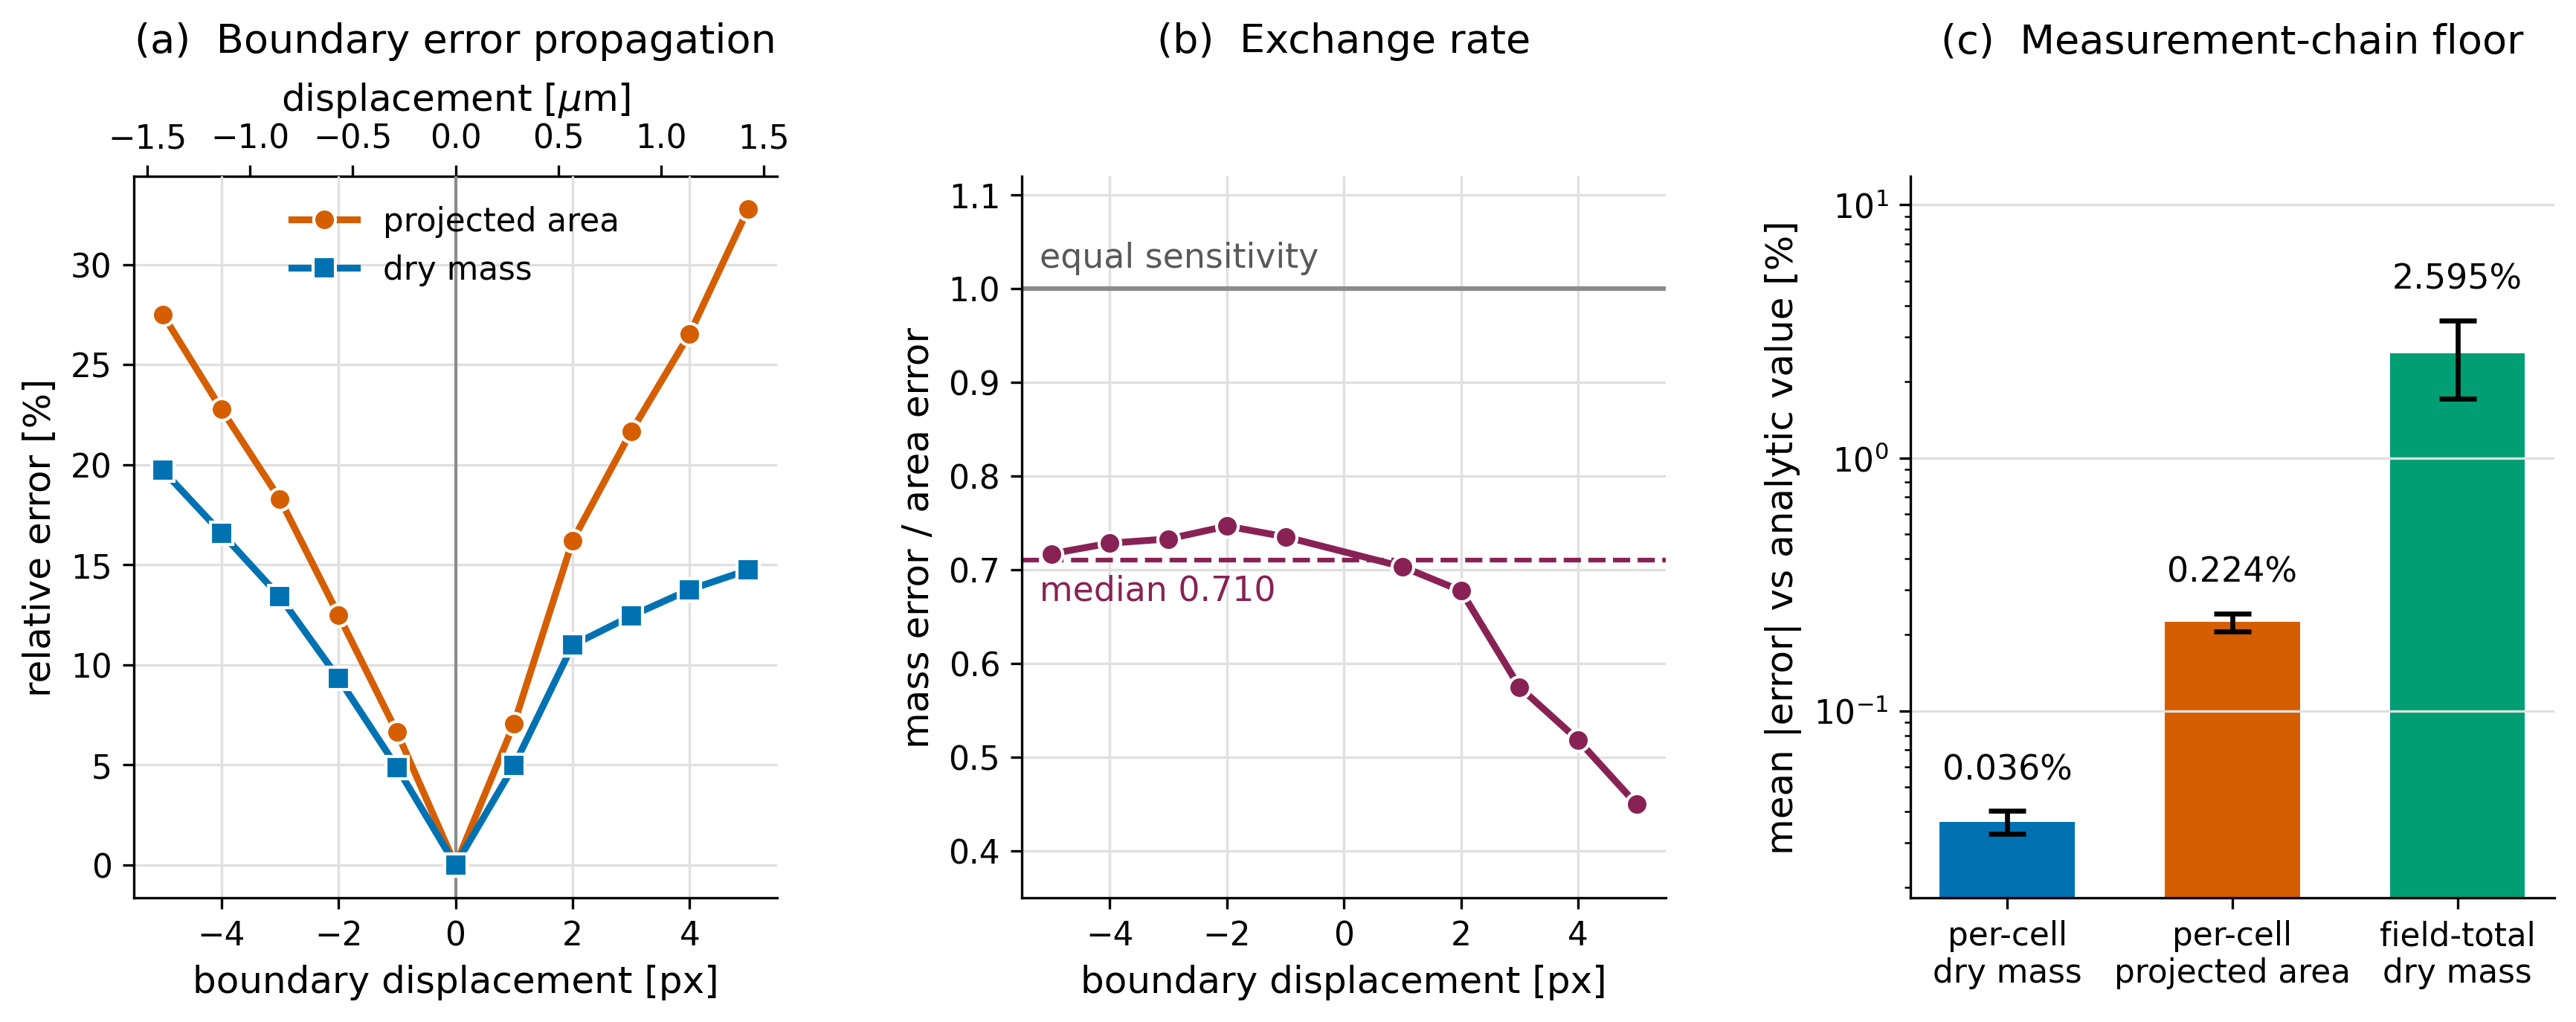
\includegraphics[width=\textwidth]{figure_8.png}
\caption{Model-free sensitivity analysis on the 113 off-axis test fields and
synthetic fields: (a) area and dry-mass error under uniform boundary
displacement of the reference masks, (b) ratio of dry-mass to area error, (c)
error of the measurement chain on three synthetic sets (mean $\pm$ SD; the
field-total bar is the mean absolute error over fields).}
\label{fig:propagation}
\end{figure}

\subsection{Computational benchmarking}
\label{sec:res-bench}

At $900\times900$ and batch 1 on an NVIDIA RTX~A5000, the baseline runs at
$12.31\pm0.12$\,ms in PyTorch FP32 and $8.42\pm0.07$\,ms in ONNX Runtime FP16,
and the Compact Baseline, which has 65\% fewer parameters, at $7.97$\,ms in ONNX
FP16 (Table~\ref{tab:efficiency}, Fig.~\ref{fig:efficiency}). Over all
benchmark sessions the $p_{99}/p_{50}$ latency ratio lies between 1.01 and
1.20. +IPP (per-cell), which shares the standard architecture, agrees with the
baseline to within 0.12\,ms except in PyTorch FP16, where its three sessions
spread from 9.31 to 10.83\,ms. The Compact Baseline changes the dry-mass MAPE by
$-0.0002$ relative to the baseline, inside the baseline's $2\times$SD of
$0.0089$; it was trained once, so the comparison is not resolvable. These are
measurements on one workstation GPU.

% Table 13: inference latency, throughput and memory on one workstation GPU.
\begin{table}[!htbp]
\centering
\caption{Computational benchmarking at $900\times900$, batch 1, on an NVIDIA
RTX~A5000. Baseline entries are mean $\pm$ SD over three benchmark sessions,
one per trained seed; the +Amplitude and Compact Baseline rows are each a
single benchmark session.}
\label{tab:efficiency}
\footnotesize
\begin{tabular*}{\textwidth}{@{\extracolsep{\fill}}llccccc@{}}
\toprule
Configuration & Runtime & \shortstack{Latency\\{[ms]}} & $p_{99}/p_{50}$ & FPS & \shortstack{Weights\\{[MB]}} & \shortstack{Peak alloc.\\{[MB]}} \\
\midrule
End-to-End Neural Baseline, $n=3$ & PyTorch FP32 & $12.31 \pm 0.12$ & $1.15 \pm 0.03$ & $81.2 \pm 0.8$ & 36.77 & 223.9 \\
9\,598\,099 par., 45.85\,GMAC & ONNX FP32 & $14.21 \pm 0.08$ & $1.08 \pm 0.06$ & $70.4 \pm 0.4$ & -- & -- \\
 & PyTorch FP16 & $9.19 \pm 0.10$ & $1.11 \pm 0.06$ & $108.9 \pm 1.2$ & 18.38 & 112.0 \\
 & ONNX FP16 & $8.42 \pm 0.07$ & $1.01 \pm 0.00$ & $118.8 \pm 0.9$ & -- & -- \\
\midrule
+Amplitude, $n=1$ & PyTorch FP32 & 12.97 & 1.13 & 77.1 & 36.81 & 223.9 \\
9\,607\,412 par., 47.87\,GMAC & ONNX FP32 & 15.45 & 1.09 & 64.7 & -- & -- \\
 & PyTorch FP16 & 11.26 & 1.12 & 88.8 & 18.40 & 111.4 \\
 & ONNX FP16 & 9.18 & 1.01 & 109.0 & -- & -- \\
\midrule
Compact Baseline, $n=1$ & PyTorch FP32 & 11.80 & 1.20 & 84.7 & 12.97 & 195.7 \\
3\,360\,403 par., 24.03\,GMAC & ONNX FP32 & 13.32 & 1.10 & 75.1 & -- & -- \\
 & PyTorch FP16 & 9.21 & 1.16 & 108.5 & 6.48 & 98.7 \\
 & ONNX FP16 & 7.97 & 1.01 & 125.4 & -- & -- \\
\bottomrule
\end{tabular*}
\tabnote{Latency: mean over 500 timed passes after 50 warm-up passes. Weights
and peak allocated memory are reported for PyTorch only.}
\end{table}


\begin{figure}[!htbp]
\centering
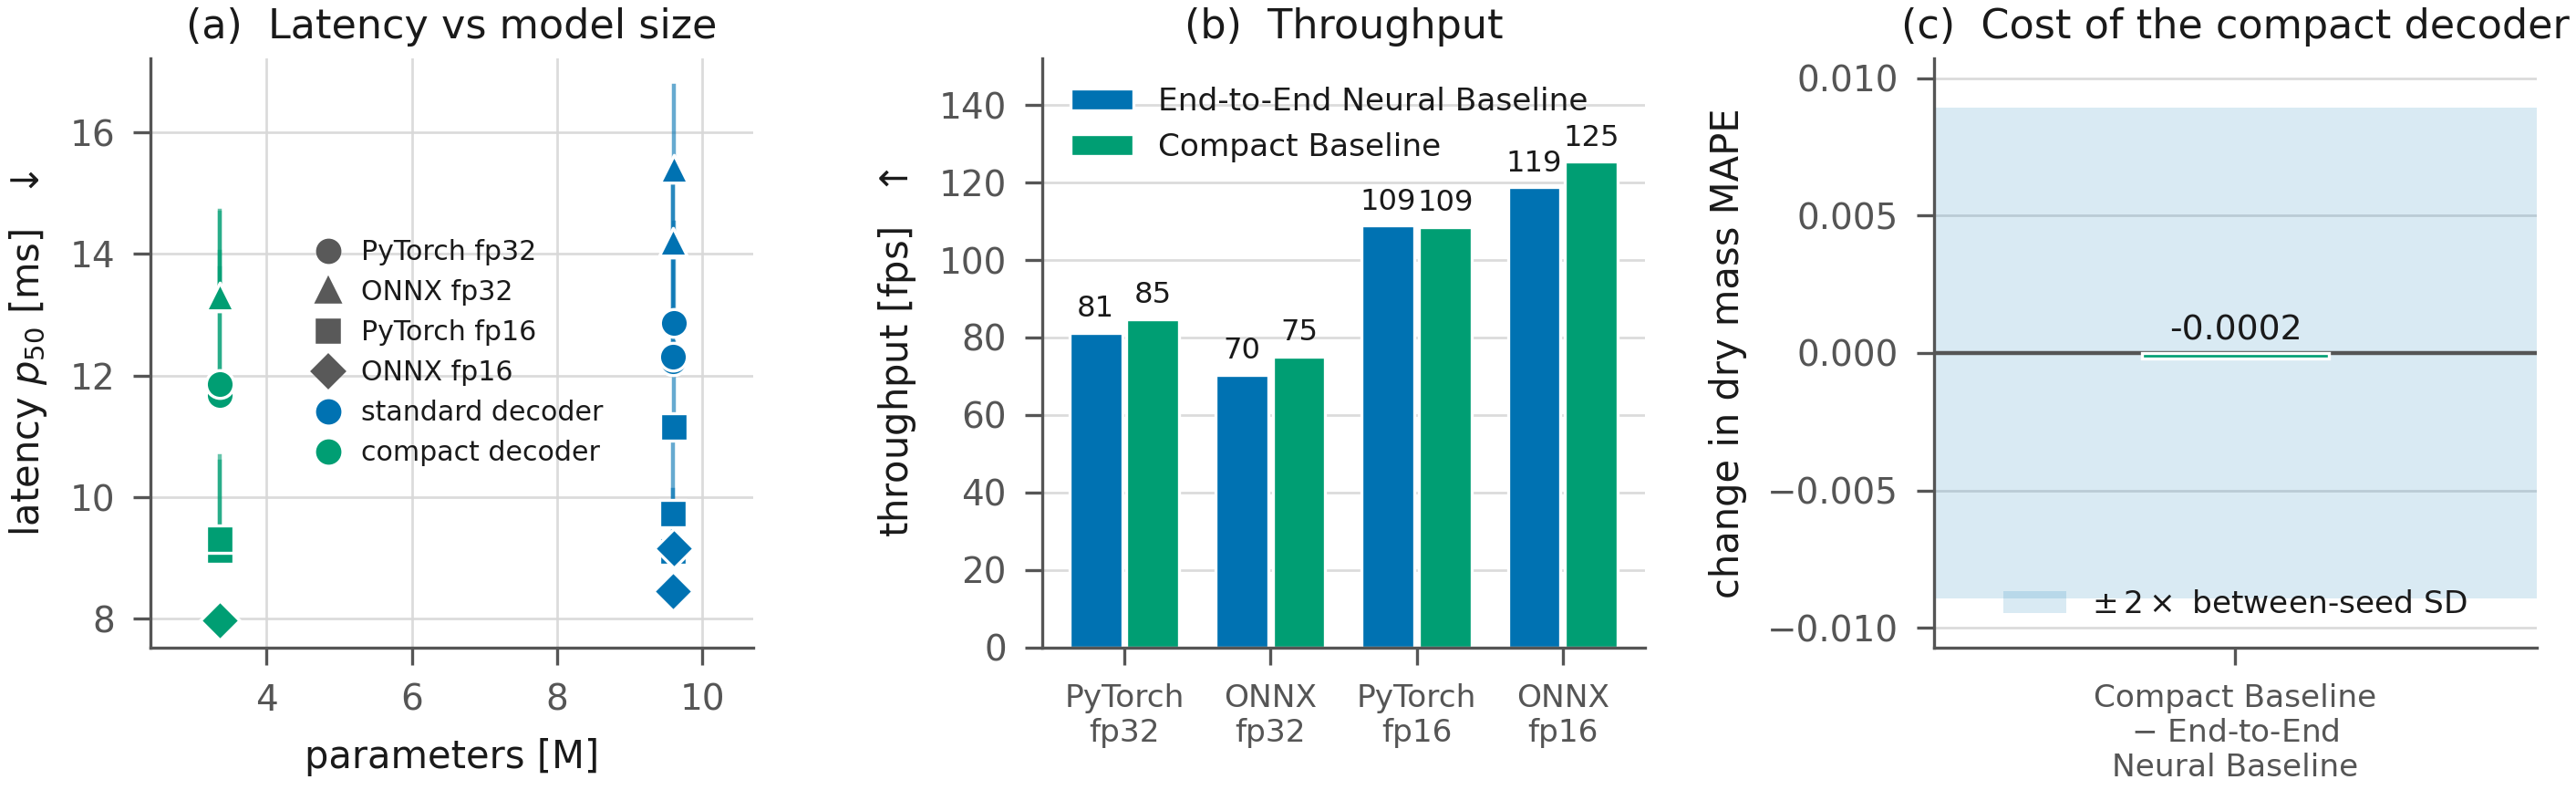
\includegraphics[width=\textwidth]{figure_9.png}
\caption{Computational benchmarking on one RTX~A5000: (a) median latency
($p_{50}$, whiskers to $p_{99}$) against parameter count, (b) throughput by
runtime and precision, (c) change in matched-cell dry-mass MAPE of the Compact
Baseline relative to the End-to-End Neural Baseline, with the baseline's
$\pm2\times$ between-seed SD band (113 off-axis test fields).}
\label{fig:efficiency}
\end{figure}

% =============================================================================
\section{Discussion}
\label{sec:discussion}

\subsection{Measurement-oriented evaluation of the end-to-end pipeline}
\label{sec:disc-baseline}

On this dataset one network that maps the raw off-axis hologram to phase and
mask gives per-cell dry-mass estimates that agree with the reference
measurements at a matched-cell MAPE of $0.174$ and a per-cell correlation of
$0.936$, closer than the tested classical configuration ($0.220$ and $0.894$).
On the 107 correctly paired fields, the in-line configuration recovers phase and
cell masks from holograms on which the tested classical in-line configuration
recovered no specimen contrast, and its matched-cell dry-mass error ($0.213$)
lies between those of the off-axis network and the off-axis classical pipeline;
with one in-line run, the comparison with the off-axis network is not
resolvable.

The closest systems in the literature reviewed in Sec.~\ref{sec:rw-joint}
predict dry mass from raw in-line holograms of plankton without a phase
image~\cite{bachimanchi2022microplankton}, reconstruct phase and virtual
fluorescence from Gabor holograms and compare measurement
distributions~\cite{park2026ai}, or chain reconstruction and detection without
per-cell phase quantities~\cite{delikoyun2025rthad}. What the present
experiments add is a paired, per-cell account of the measurement for one joint
network on experimental off-axis and in-line holograms, next to the fraction of
reference cells the account covers and a split of the error into domain and
phase. The comparison with those systems is qualitative; they use other
specimens, other supervision and other instruments, and none of them was run on
the data used here.

For learned holographic pipelines whose purpose is a per-cell quantity, the
experiments point to three reporting practices. The per-cell error should be
computed on matched cells and stated together with recall, because on this
dataset the coverage-adjusted error ($0.510$) is almost three times the
matched-cell error ($0.174$). Segmentation overlap should not stand in for
measurement accuracy, because a Dice of $0.974$ is compatible with a 5\% mass
error per cell. And the handling of cells at the field boundary should be part
of the reference definition, because it decides a large part of the recall.

\subsection{Why overlap metrics and measurements diverge}
\label{sec:disc-divergence}

Against the tested classical pipeline, Dice ($0.825$ and $0.834$) and projected
area MAPE ($0.158$ and $0.157$) are close, while the matched-cell dry-mass MAPE
differs ($0.220$ and $0.174$). The decomposition shows how the two errors are
structured. For matched cells the network's domains enclose almost the same
reference phase integral as the reference domains (domain factor $1.002$), and
its error sits in the phase factor ($0.929$); the classical pipeline instead
shows opposing domain and phase deviations ($0.966$ and $1.014$). The lower
in-cell phase MAE of the network ($0.269$ against $0.311$\,rad) is consistent
with this split.

The model-free analysis gives the scale of the decoupling between overlap and
measurement. A one-pixel boundary displacement leaves Dice at $0.974$ but
changes area by about 7\% and dry mass by about 5\%, so segmentation scores in
the range reported here are compatible with measurement errors of ten percent
or more. The observed matched-cell area error ($0.157$) is of the same order as
the area change produced by a uniform two-pixel displacement ($-12.3\%$
inward, $+15.0\%$ outward). The displacement analysis applies a uniform shift
and does not decompose the observed error, so this is a comparison of scale,
not an attribution. Dry mass changes less than area under the same
displacement (median ratio $0.71$), which is consistent with the phase being
low at the cell periphery. Classical DHM analyses report the same sensitivity
from other directions: Bai \emph{et al.} attribute part of an apparent volume
increase to phase halos that place the segmented boundary outside the
cell~\cite{bai2026macrophage}, and Kyeremah \emph{et al.} describe
morphological red-blood-cell features as sensitive to boundary
precision~\cite{kyeremah2025malaria}. The learned reconstructions reviewed in
Sec.~\ref{sec:rw-recon} are mostly scored with SSIM, PSNR or pixel error. By
the numbers above, an image or overlap score in the range typically reported
does not bound the per-cell measurement error.

\subsection{Detection coverage and boundary objects}
\label{sec:disc-coverage}

The matched-cell MAPE of $0.174$ describes the roughly 1890 of 3186 reference
cells that were detected and matched. With recall $0.593$, the
coverage-adjusted error is $0.510$ and the field-total dry mass is low by about
16\%, and the model also reports on average $337$ false-positive cells per run,
which enter the field totals but no per-cell error. The field-level domain
factor ($0.897$) carries the same deficit. The location stratification shows
that the missed cells are concentrated in one population: interior reference
cells are recalled at $0.912$ and edge instances at $0.212$. Edge instances
include cells truncated by the field of view and boundary regions that the
reference masks retain because the border-removal step, as configured, has no
effect after closing.

The field totals depend on how detection and measurement errors combine, and
here the ordering of the two pipelines reverses: the classical pipeline has the
higher matched-cell error but the lower field-total error ($0.109$ against
$0.163$). Its field-level domain and phase factors deviate in opposite
directions ($0.857$ and $1.055$), which indicates a compensatory error
structure in which part of the domain deficit is offset by a raised phase. A
field-total error alone would not separate this case from one in which both
domain and phase are close to the reference.

Cells truncated by the field of view have physically incomplete area and dry
mass, so whether they belong in a per-cell reference is a methodological
choice. Two of the DHM studies we reviewed remove them before analysis:
HoloPhaseNet discarded cells at the border of the phase
image~\cite{jaferzadeh2022holophasenet}, and a SAM-based red-blood-cell
pipeline removed cells touching the image edge~\cite{numata2024rbcsam}. Some of
the low overall recall may therefore reflect objects that a different labelling
rule would exclude. The edge instances were not classified individually, so the
size of that share is not known. The stratification was not used to redefine
any reported metric: recall and the coverage-adjusted error are those of the
full reference population.

\subsection{Measurement-aware objectives}
\label{sec:disc-mawo}

Three observations are direct. Both integrated-phase terms increased the
matched-cell dry-mass error by more than twice the pooled between-seed standard
deviation, and neither changed the field-total error by a resolved amount. The
matched-cell increase is resolved among interior cells and not among edge
cells. And the per-cell term added about 119 false-positive cells per run and a
resolved increase of the field-level domain factor, whereas the image-level
term did not change the false-positive count.

One property of the formulation bears on the last observation. $\Lippc$ sums
only over reference instances, so predicted foreground outside them contributes
nothing to it, whereas $\Lippi$ sums over the whole crop and so includes the
phase under any false-positive foreground. The difference in false positives
between the two terms is consistent with this, but the experiment does not
isolate it as the cause. The formulation also admits a receding foreground with
a raised phase as a way to satisfy $\Lippc$ (Sec.~\ref{sec:obj-mawo}); the
unchanged matched-cell domain factor shows that the trained models did not take
this route.

Two further possibilities were not tested. The first concerns the labels. The
reference mask is a deterministic function of the reference phase, so when
$\Lphase$ and $\Lseg$ are both well fitted, the quantity the integrated-phase
terms constrain is already largely determined by them. An additional soft
constraint on it may then add little information while adding gradient to the
segmentation decoder, measured at initialisation as about $0.37$ of the
segmentation gradient at $w=1$. If this is the mechanism, the terms could
behave differently with segmentation labels that are independent of the phase
target, such as masks derived from fluorescence acquired on the same
field~\cite{park2025holofluonet}. The second concerns the edge objects, which
the per-cell term includes as integration domains during training. About half of
the additional false positives under that term lie within 15\,px of the field
boundary, but the resolved increase in measurement error is among interior
cells. Whether edge objects affect training in other ways would require
retraining with regenerated masks.

The result is specific: these terms, at these weights, with these labels and
this architecture, did not reduce the per-cell measurement error. It does not
show that measurement-aware objectives cannot help, and it does not establish
how the terms behave with other models or datasets. The two terms were compared
at equal coefficients without matching their gradients. The +Area, +BGA,
amplitude and forward-model configurations were trained once each, and single
runs cannot exclude small effects in either direction. In the literature we
reviewed, the only case where a measurement enters training is as a regression
target learned from simulation~\cite{bachimanchi2022microplankton}, so these
results cannot be set against a previous test of the same kind of term on
experimental data.

\subsection{What the forward-model term constrains}
\label{sec:disc-fwd}

The forward-model term is the only component that relates the prediction to the
recorded hologram through a model of image formation. Its behaviour differs
between the geometries. In-line, the reference-phase residual has a clear
minimum at the recording distance on every scanned field, so under the
implemented operator the residual identifies $z$. Off-axis, it did not: the
pooled minimum lies at the same grid point, but two of the four fields have
their best distance at the ends of the scanned range. This is consistent with
Eq.~\eqref{eq:offaxis}, in which the carrier encodes the phase at any distance,
so the off-axis hologram changes little with $z$; the scan does not test that
explanation directly.

Near the reference phase, the residual is insensitive to the phase scale in both
geometries. A 10\% rescaling raises it by less than the configured tolerance of
$0.01$ off-axis ($0.00035$) and in-line ($0.0043$), although in-line the change
has the same sign on 30 of the 32 fields. Off-axis, the global aberration
surface leaves most of the variance unexplained even for the reference phase,
and per-field surfaces, fitted against each field's reference phase, leave much
less: on the 112 test fields that have a per-field surface, the residual is
$0.893$ with the global surface and $0.391$ with per-field surfaces. This is
consistent with
field-specific structure that the global surface does not represent accounting
for part of the unexplained variance. With the term trained at $w=0.02$, the
+Fwd configurations did not reach a lower residual ratio than the baseline, and
their in-cell phase error was higher; as single runs these differences are not
resolvable.

The holographic forward-model methods discussed in Sec.~\ref{sec:rw-fwd} use
in-line intensity with a distance that is fixed or obtained by
autofocusing~\cite{wang2020physennet,huang2023gedankennet,galande2024hdphysnet}.
The free-distance configuration tested here treats the distance as an unknown
calibration parameter of an off-axis model, the partially known case in the
terminology of Ongie \emph{et al.}~\cite{ongie2020deep}. These results
characterise the implemented operator, evaluated on four fields per geometry
for the distance scan and on 32 to 113 fields for the phase-sensitivity probes.
They do not establish how other forward-model formulations would behave.

The amplitude output fits into the same picture. The network produces an
amplitude map that agrees with the classical amplitude reference more closely
than the unit-amplitude assumption, and this map completes the predicted
complex field used by the forward model. Dry mass does not use the amplitude,
so no direct effect on the measurement is expected; with single runs, none
could be resolved.

% =============================================================================
\section{Limitations}
\label{sec:lim}

All segmentation, detection and matched-cell measurement results are relative
to masks derived from the reference phase by a fixed thresholding rule. They do
not measure agreement with an independent delineation, and the scores against
the provisional membrane-derived masks are much lower. The Otsu level also
varies with drug condition, so between-condition morphology comparisons made
with these labels would partly reflect the label definition; no such
comparison is reported here. As configured, the rule keeps truncated and
boundary objects, and changing it would change the reference and require
re-evaluating every configuration. The reference phase is itself a processed
reconstruction whose exact processing is not known to us, and the amplitude
reference is the modulus of a classical reconstruction; neither is an
independent physical measurement.

The hologram crop origin was determined empirically, on validation fields, by
registration of a classical reconstruction to the reference phase. Its median
residual on the test fields is below one pixel, but a per-field scatter of
about $\pm2$--$3$\,px (5--95\% range) remains, so on some fields the network
input and the phase target are offset by a few pixels.

The in-line result rests on a single training run, evaluated on 107 test
fields, after excluding the 50 fields whose in-line frames do not correspond to
their reference. The classical in-line reconstruction was run at one distance
and with one algorithm.

Only the baseline and the two integrated-phase configurations have three runs.
All other comparisons are single runs and are reported as not resolvable. The
image-level term was run at the per-cell term's coefficient without matching
its gradient magnitude. The location stratification and the mass-error
decomposition were carried out after training.

The forward-model conclusions apply to the implemented operator (scalar
angular-spectrum propagation, a global order-5 aberration surface, a six-term
radiometric fit off-axis) and to a term weight of $0.02$. The distance scan
covers four validation fields per geometry, and the per-field aberration
surfaces used in one sensitivity probe are fitted against the reference phase.

All fields come from one instrument and three adherent cancer cell lines, and
generalisation to other instruments, magnifications or cell types is untested.
Computational cost was measured on one workstation GPU. The model outputs are
predicted at half resolution and bilinearly upsampled. Absolute masses depend
on $\alpha=0.2$\,mL/g, the value used by the acquiring group, within a
literature range of $0.173$--$0.215$\,mL/g~\cite{zhao2011,chaumet2024};
relative results do not.

% =============================================================================
\section{Conclusions}
\label{sec:conclusions}

A network that maps a raw off-axis hologram to quantitative phase and a cell
segmentation measured per-cell dry mass on this dataset with a matched-cell
MAPE of $0.174$, against $0.220$ for the tested classical configuration, at
similar Dice and projected-area error. For matched cells the network's error
lies in the predicted phase level rather than in the predicted cell domain. For
the full reference population, detection coverage is a larger limitation than
the measurement error of detected cells (coverage-adjusted dry-mass error
$0.510$), and the missed cells are concentrated among boundary objects that the
phase-derived labels retain. Field totals rank the two pipelines the other way,
and the decomposition indicates a compensatory error structure in the classical
pipeline. On correctly paired in-line holograms, a single training run recovered
phase where the tested classical in-line reconstruction did not.

Terms designed to preserve the integrated phase per cell or per image increased
the matched-cell dry-mass error under the evaluated setup without a resolved
change in the field-total error, and neither an area term, a boundary-alignment
term, other weights, an amplitude output nor a forward-model term brought it
below the baseline in single runs. Under the implemented operator, the
forward-model residual identified the propagation distance in-line, did not
constrain it off-axis, and did not resolve a 10\% change of the phase scale in
either geometry. A one-pixel boundary shift that leaves Dice at $0.974$ changes
dry mass by about 5\%. Testing whether measurement-aware objectives help when
segmentation labels are independent of the phase target, and whether a more
complete forward model makes hologram consistency informative off-axis, are the
direct next experiments.


% =============================================================================
{\small
\bibliographystyle{unsrt}
\bibliography{references}}

\end{document}
